%%%% Proceedings format for most of ACM conferences (with the exceptions listed below) and all ICPS volumes.
\documentclass[sigconf]{acmart}
\usepackage{algorithm}
\usepackage[export]{adjustbox}
\usepackage[noend]{algpseudocode}
%%%% As of March 2017, [siggraph] is no longer used. Please use sigconf (above) for SIGGRAPH conferences.

%%%% Proceedings format for SIGPLAN conferences 
% \documentclass[sigplan, anonymous, review]{acmart}

%%%% Proceedings format for SIGCHI conferences
% \documentclass[sigchi, review]{acmart}

%%%% To use the SIGCHI extended abstract template, please visit
% https://www.overleaf.com/read/zzzfqvkmrfzn

%
% defining the \BibTeX command - from Oren Patashnik's original BibTeX documentation.
\def\BibTeX{{\rm B\kern-.05em{\sc i\kern-.025em b}\kern-.08emT\kern-.1667em\lower.7ex\hbox{E}\kern-.125emX}}
    
% Rights management information. 
% This information is sent to you when you complete the rights form.
% These commands have SAMPLE values in them; it is your responsibility as an author to replace
% the commands and values with those provided to you when you complete the rights form.
%
% These commands are for a PROCEEDINGS abstract or paper.
\copyrightyear{2018}
\acmYear{2018}
\setcopyright{acmlicensed}
\acmConference[Woodstock '18]{Woodstock '18: ACM Symposium on Neural Gaze Detection}{June 03--05, 2018}{Woodstock, NY}
\acmBooktitle{Woodstock '18: ACM Symposium on Neural Gaze Detection, June 03--05, 2018, Woodstock, NY}
\acmPrice{15.00}
\acmDOI{10.1145/1122445.1122456}
\acmISBN{978-1-4503-9999-9/18/06}

%
% These commands are for a JOURNAL article.
%\setcopyright{acmcopyright}
%\acmJournal{TOG}
%\acmYear{2018}\acmVolume{37}\acmNumber{4}\acmArticle{111}\acmMonth{8}
%\acmDOI{10.1145/1122445.1122456}

%
% Submission ID. 
% Use this when submitting an article to a sponsored event. You'll receive a unique submission ID from the organizers
% of the event, and this ID should be used as the parameter to this command.
%\acmSubmissionID{123-A56-BU3}

%
% The majority of ACM publications use numbered citations and references. If you are preparing content for an event
% sponsored by ACM SIGGRAPH, you must use the "author year" style of citations and references. Uncommenting
% the next command will enable that style.
%\citestyle{acmauthoryear}

%
% end of the preamble, start of the body of the document source.
\begin{document}

%
% The "title" command has an optional parameter, allowing the author to define a "short title" to be used in page headers.
\title{Runtime level failure detection and propagation in HPC systems}

%
% The "author" command and its associated commands are used to define the authors and their affiliations.
% Of note is the shared affiliation of the first two authors, and the "authornote" and "authornotemark" commands
% used to denote shared contribution to the research.
\author{Dong Zhong}
\email{dzhong@vols.utk.edu}
\orcid{1234-5678-9012}
\authornotemark[1]
\affiliation{%
  \institution{The University of Tennessee}
  \streetaddress{P.O. Box 1212}
  \city{Knoxville}
  \state{TN}
  \postcode{43017-6221}
}

\author{George Bosilca}
\affiliation{%
  \institution{The University of Tennessee}
  \city{Knoxville}
  \state{TN}}
\email{larst@affiliation.org}

\author{Aurelien Bouteiller}
\affiliation{%
  \institution{Inria Paris-Rocquencourt}
  \city{Rocquencourt}
  \country{France}
}

%
% By default, the full list of authors will be used in the page headers. Often, this list is too long, and will overlap
% other information printed in the page headers. This command allows the author to define a more concise list
% of authors' names for this purpose.
\renewcommand{\shortauthors}{Dong and Aurelien, et al.}

%
% The abstract is a short summary of the work to be presented in the article.
\begin{abstract}
As the scale of High Performance Computing (HPC) system continues to grow, with more and more nodes deployed, mean-time-to-failure (MTTF) of those HPC systems is dramatic impacted (become lower and lower/drops). In order to efficiently run long time computing job on these systems, fault tolerance become a prime challenge/technology. In this paper, we present the design and implementation of an efficient runtime-level failure detection and propagation strategy targeting exascale systems. The detection is able to detect both node failure and process failure. A ring topology is maintained by allowing one node sending and receiving periodically heartbeat to/from another node to detect a node failure(observing another single node). For process failure each host node (is in charge of monitoring) monitors its children processes. The propagation use a reliable broadcast method over a binomial graph(an arbitrary communication topology) to distribute error message to applications, guarantees a logarithmic propagate time. We focus primarily on the most widely used programming paradigms PMIx Reference RunTime Environment(PRRTE), the algorithms and strategies proposed have a larger scope of most distributed programming environment. Experiments on different machines successfully demonstrated the algorithm performs well.
\end{abstract}

%
% The code below is generated by the tool at http://dl.acm.org/ccs.cfm.
% Please copy and paste the code instead of the example below.
%
\begin{CCSXML}
<ccs2012>
 <concept>
  <concept_id>10010520.10010553.10010562</concept_id>
  <concept_desc>Computer systems organization~Embedded systems</concept_desc>
  <concept_significance>500</concept_significance>
 </concept>
 <concept>
  <concept_id>10010520.10010575.10010755</concept_id>
  <concept_desc>Computer systems organization~Redundancy</concept_desc>
  <concept_significance>300</concept_significance>
 </concept>
 <concept>
  <concept_id>10010520.10010553.10010554</concept_id>
  <concept_desc>Computer systems organization~Robotics</concept_desc>
  <concept_significance>100</concept_significance>
 </concept>
 <concept>
  <concept_id>10003033.10003083.10003095</concept_id>
  <concept_desc>Networks~Network reliability</concept_desc>
  <concept_significance>100</concept_significance>
 </concept>
</ccs2012>
\end{CCSXML}

\ccsdesc[500]{Computer systems organization~Embedded systems}
\ccsdesc[300]{Computer systems organization~Redundancy}
\ccsdesc{Computer systems organization~Robotics}
\ccsdesc[100]{Networks~Network reliability}

%
% Keywords. The author(s) should pick words that accurately describe the work being
% presented. Separate the keywords with commas.
\keywords{fault tolerance, failure detection, reliable broadcast, message propagation, HPC runtime system}

%
% This command processes the author and affiliation and title information and builds
% the first part of the formatted document.
\maketitle

\section{Introduction}
The drive to produce more and more powerful supercomputers leads to HPC platforms/systems consist millions of cores distributed over hundreds of thousands of nodes, it is becoming increasingly imperative to adopt fault tolerance and resilient features to applications and runtime environments. Efforts toward fault tolerance has been attempted by researchers at application level. 

A runtime environment support distributed HPC applications operating in heterogeneous environment, the system provide service for managing processes launching, deployment and monitoring, also providing interaction and communication infrastructures for hosts and parallel applications. 

A resilient runtime environment must have the capability of continuing the job execution even with failures, and also be able to detect failure and distribute the fault information to the applications with minimal disturbance to the whole system.  

TODO:
Detection and propagation ?

\section{Related work}
In this section, we survey related work on runtime environments, failure detectors and reliable broadcast algorithms to propagate fault information.

\subsection{Runtime systems}
A wide range of approach to the problem of exscale distributed computing runtime environments have been studied, each primarily emphasizing a particular key aspect of the over all problem. MPICH provides several runtime environments such as MPD\cite{Butler00}, Hydra\cite{MPICH14}, Gforker. MPD connect nodes through a ring topology which is not resilient, two node failures is enough to separate nodes in two separate groups that prevent communication with one another. Another drawback is this approach has proved to be non-scalable. Hydra scale well for large number of processes on a single node and efficient interaction with hybrid programming models that combine MPI and threads. The Open MPI runtime environment, ORTE\cite{Castain05}\cite{Jeffrey12} provide not only the required message passing API, but also an accompanying run-time system to launch, monitor, and kill parallel jobs. Also ORTE connect daemons through various topology, however the communication is not reliable. However, all those runtimes are limited to MPI application, and PRRTE work has the capability to run MPI jobs more scalability, but also supports applications utilize more than one programming model, such as an MPI application that also uses OpenMP. 

\subsection{Failure detection}
Research in the ares of failure detection has been extensively studied. Chandar and Toueg\cite{Chandra96} proposed the first unreliable failure detector oracle that can solve consensus and atomic broadcast problem for reliable distributed systems. Many implementations\cite{Wei02}\cite{Larrea00}\cite{Kawazoe97} are based on this oracle work using all to all communication where every node periodically sends heartbeats to all nodes. However those implementations are not scalable for lager systems with hundreds of thousands of nodes. The technique gossip-style protocols\cite{van98} \cite{Ranganathan01}\cite{Gupta01}\cite{Abhinandan02}  (where nodes pick some other nodes to monitor and exchange information) become popular approach for failure detection in order to scale up. However gossip methods do not work well with large number node crashes, also detecting a specific failure can potentially take a fairly long time. Furthermore, gossip method still has the disadvantage of redundant failure messages decreases the scalability.

Recently, Application lvl ulfm @ George sc16 one port model 
TODO:

\subsection{Reliable broadcast}
Reorder BMG.depth is the same but average is lowers. cause system noisy less cause message reach faster -> less propagation.

Notable efforts have been made for fault-tolerant communication based on existing logical network topologies. Fully connected topology is perfect in the sense of fault tolerant but cannot be scalable. A circular topology is good for scalability but suffers from multiple node failures.  
A more recent effort to introduce is k-nomial Graph \cite{Angskun07}\cite{Pava11}, the key-concept of fault-tolerant broadcasting is diameter of the topology, which is defined the longest shortest path between any two nodes in the graph. Binomial Graph has scalable capability properties with reasonable degree, regular graph and lowest diameter. However when doing a reliable broadcast with message forwarding, this method use a fixed sending sequence to all the neighbours. Our work use Binomial Graph with a reordering strategy when sending and forwarding messages, which means lower average reroute hops and message traffic density.

\section{Design and implementation}

In this section, we describe the design of Resilient PRRTE and we provide rationale for our design decisions. Also we give a detailed description about the implementation.

\begin{figure}[h]
  \centering
  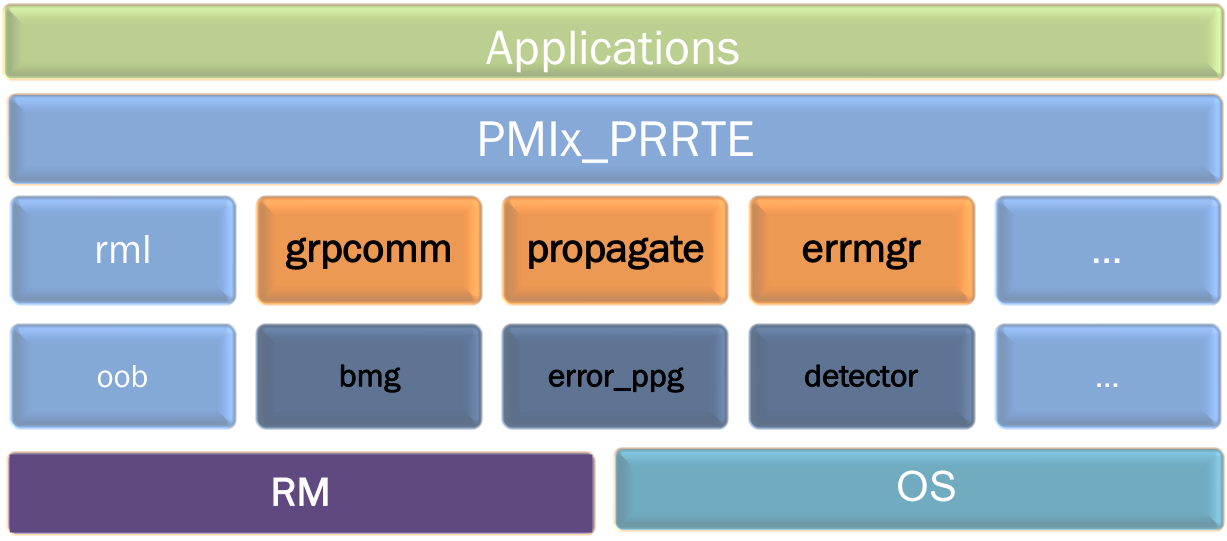
\includegraphics[width=\linewidth]{PMIx_PRRTE.png}
  \caption{Resilient PRRTE component architecture. The orange boxes represent the component we mainly use to add the resilient features. The dark blue colored boxes are the new modules}
\end{figure}

\begin{figure}[h]
  \centering
  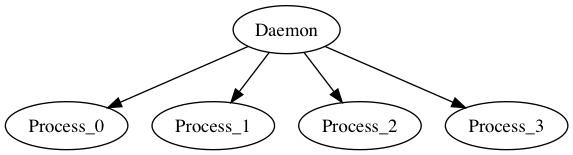
\includegraphics[width=\linewidth]{test.png}
  \caption{Notify the error locally}
\end{figure}
\subsection{Model}
PRRTE originated as OpenRTE \cite{Castain05} which is based upon Module Component Architecture (MCA) developed under the Open MPI project. Then spun off to its own effort as a ``\verb|shim|`` between the application and the host environment that includes full support for the PMIx \cite{CASTAIN18} - an abstract set of interfaces by which not only applications and tools can interact with the resident system management stack (SMS), but also the various SMS components can interact with each other. 

PRRTE provides an easy way of launching, running and monitoring PMIx-based applications outside of a PMIx-enabled environment on distributed systems. The PRRTE overall architecture is out the scope of this paper, but we still want to mention some feature embraced by it. First of all, PRRTE's very first feature is Job control and Monitoring \cite{Ralph15} and  which enables the application and SMS to coordinate the response to failure: termination of the job or a subset of processes, request replacement of nodes and processes, or continue execution at a lower setting. This provides the foundation of resilience strategy of our work. Another important feature is the PMIx Event Notification \cite{Ralph002} : the resource manager or server can notify the application of events, the application processes can notify their server or SMS of issues. This provides the channel for locally propagation of error messages. Resilient PRRTE mainly embraces two new features of failure detection and reliable broadcast for messages propagation globally and locally. We will give a detail introduction of the two features in the following part.

\subsection{Detection of process and node failure/Error management}

\begin{table}
  \caption{Parameters and notations}
  \label{tab:parameters}
  \begin{tabular}{ccl}
    \toprule
    Symbol & Description \\
    \midrule
    \texttt \bf N & Number of Daemon/nodes \\
    \texttt Id & The identifier of a Daemon \\
    \texttt LIST\{ID\} & List of known failed daemons' ID \\
    \texttt  $\delta$ & Heartbeat period \\
    \texttt  $\eta$ & Timeout for assuming a daemon failure\\
    \bottomrule
  \end{tabular}
\end{table}

\begin{figure}
\centering
\begin{minipage}{.23\textwidth}
  \centering
  
\includegraphics[width=\linewidth]{ring_detector.png}
  \captionof{figure}{Ring topology}
  \label{fig:Ring}
\end{minipage}%
\begin{minipage}{.23\textwidth}
  \centering
  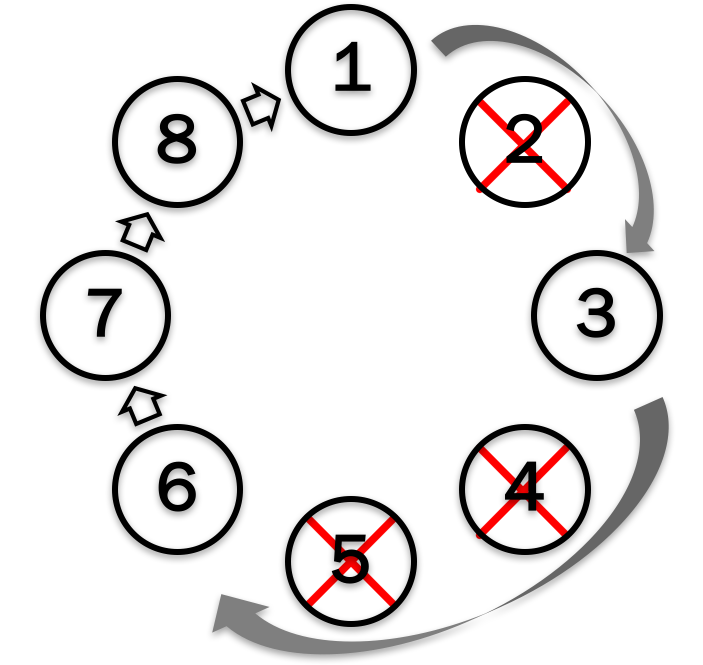
\includegraphics[width=\linewidth]{reconnet_cross.png}
  \captionof{figure}{Reconnect with failures}
  \label{fig:Reconnect Ring}
\end{minipage}
\end{figure}
We provide strategy to detect both process failure and node failure in different ways. The OpenRTR Daemon's Local Launch Subsystem(odls) is responsible for launching and monitoring local processes that are intended to launch the target applications' executable. Before the children processes execute the targets' executable, it need to set affinity of children processes according to a complex series of rules. This binding may fail in a myriad of different ways, the children processes will send a message to the parent indicating what happened (rendered error message) and the parent will read the message and analyze if this is a process failure and the use the runtime system's reporting mechanisms to display this error globally. 

For a general distributed system, nodes can communicate to any other nodes by sending message through communication channels. We arrange all N nodes to a logistic ring topology as in figure 2, which means, each particular node \textbf{\textit{p}} has a observer and a predecessor in the ring. The predecessor will send periodic heartbeat messages to \textbf{\textit{p}} with the period of T, at the same time \textbf{\textit{p}} will send heartbeat messages to its observer. For each node it emits heartbeats $m_1$, $m_2$, ... at time ${\tau_1}$, ${\tau_2}$, ... to its observer \textbf{\textit{q}}. Let ${\tau_i^'}$ = ${\tau_i}$ + $t$. At any time \textbf{\textit{t}} $\in$ [${\tau_i^'}$, ${\tau_+1^'}$), \textbf{\textit{q}} believe \textbf{\textit{p}} is alive if it receive message $m_i$ or higher. Otherwise, \textbf{\textit{q}} suspect \textbf{\textit{p}} is failed, \textbf{\textit{q}} will prepare error information of \textbf{\textit{p}} and propagate this information. 

When the observer detects the predecessor is failed, there are two major steps we do. First we need to reconnect the ring topology as in figure 3, the observer will search its own known failed list and figured the first alive node \textbf{\textit{nq}} preceding in the ring, it set \textbf{\textit{nq}} as its predecessor and then send a request to \textbf{\textit{nq}} for being the new observer. The second step is failure propagation: the observe need to get access to the job's global mapping and binding information and find out all those processes hosted on predecessor node. After we get the list of all those affected processes and node, the observer call the propagation component to delivery this message on node level to its neighbours, then observer will notify its local processes. Then, the observer updates its local known failure List\{\textit{ID}\}. For all those nodes who received the notification, each node need to forward this information, maintain its own List\{\textit{ID}\} and notify locally. 

\subsection{Failure propagation}
For broadcasting we use the scalable and fault tolerant topology binomial graph (BMG)\cite{Angskun07}. BMG has good fault-tolerant properties such as optimal connectivity, low fault-diameter, strongly resilient and good optimal probability in failure cases. In order to continuing the job execution rather than aborting, we need to let all participated nodes and applications aware of failures, the three major mechanisms are 
\begin{enumerate}
  \item Observer fetch error information of failed node. Start the propagation globally by calling group communication component for broadcasting.
  \item Observer node broadcast the information to all its local children. 
  \item All nodes forwarding the message upon receiving to make the broadcast reliable. Make sure all alive nodes receive the information at least once. 
\end{enumerate}

\begin{algorithm}
\caption{Reliable broadcast algorithm }
\textbf{\textit{N}} \Comment{Number of alive nodes}\newline
\textbf{List\{$EID$\}} \Comment{Local list of known error processes' identifier}\newline
\textbf{\textit{msg}} \Comment{Message packed with jobid, process identifiers and state}\newline
\textbf{\textit{flag}} \Comment{Boolean flag indicating forward the message or not}\newline
\textbf{List\{$AID$\}} \Comment{Processes identifiers' hosted on failed daemon identifier }\newline

\begin{algorithmic}[1]
\Procedure{Broadcast}{ $i, N, msg$ }\Comment{Daemon \textbf{i} send error message to all its neighbours}
\For{ $k \gets 0$ to $\log_2 N$ }\Comment {Order not fixed}            
     \State {\textbf{i} send \textbf{msg} to  ( ($N$ + i + $2^k$) \textbf{mod} {N} ) }
     \State {\textbf{i} send \textbf{msg} to  ( ($N$ + i - $2^k$) \textbf{mod} {N} ) }
\EndFor
\EndProcedure
\end{algorithmic}

\begin{algorithmic}[1]
\Procedure{Forwarding}{ $flag, msg$ }\Comment{Daemon \textbf{j} receives msg, forwarding and notify locally }
\If {$flag == true$}
    \State Broadcast( $j, N, msg$ )
    \State Update \textbf{List\{$EID$\}}
    \State Notify locally
\EndIf
\EndProcedure
\end{algorithmic}

\begin{algorithmic}[1]
\Procedure{Start propagation}{ $job, Eid, state$ }\Comment{Daemon \textbf{j} start propagation }
\If {( $Eid$ $\notin$ List\{$EID$\} )}
    \State Add $Eid$ to $msg$
    \State Get \textit{AID} and adde to $msg$
    \State Broadcast( $j, N, msg$ )
    \State Add $Eid$ \textit{AID} to List\{$EID$\}
\EndIf
\EndProcedure
\end{algorithmic}

\end{algorithm}

Group communication use out-of-band non-blocking peer to peer as the basic message exchange mechanism, we assume the communication latency from any two directly connected nodes with same message size are equivalent. For node level broadcast, each node send message to all its neighbours  as in BMG topology, message from any node we follow the sequence as in binomial spanning tree by which means that any node in BMG can always be delivered within $O(log_2^N)$ steps. 

\begin{figure}
  \centering
  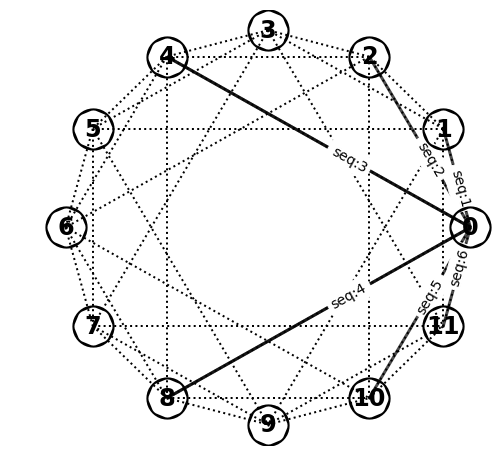
\includegraphics[width=\linewidth]{bmg_origin.png}
  \caption{Binomial graph with 12 nodes}
\end{figure}
\begin{figure}
  \centering
  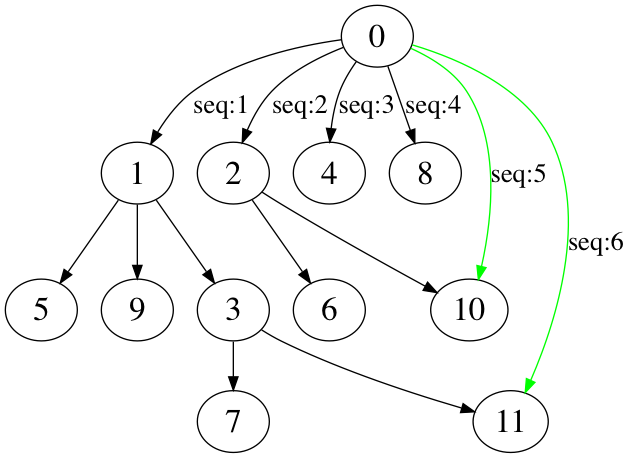
\includegraphics[width=\linewidth]{reorder_seq.png}
  \caption{Broadcast using binomial spanning tree from node 0, extra messages to neighbours are colored in green }
\end{figure}
Figure 5 shows the BMG with 12 nodes with, node 0 start the propagation and send messages to all its six neighbours with the sequence marked. And Figure 6 shows the a spanning tree for broadcast originated from node 0 also with extra messages colored green for resilient purpose. Those extra green messages balanced the trade-offs between high-radix trees that allow for more parallelism at each level in the tree and more network connection, and lower-radix deeper communication trees with reduced network congestion. The advantages of this new broadcast algorithm:
\begin{enumerate}
  \item Excellent network connection with higher parallelism: message to node \{10, 11, 7\} could arrive from any forwarding nodes at earlier time stamp than routed from spanning tree, this decrease the height of the tree, the average latency and the maximum of notification delay are smaller.
  \item Limited network connection: maintains the upper bound of broadcast to $O(log_2^{12})$. 
\end{enumerate}
For inter-node notification, children process subscribe to a event handler with specific error code and triggered by the notification function. 
Application can register to multiple events.

\section{Experiment Evaluation}

\subsection{Experiment Setup}
The experiment are conducted on two different machines, the first one is our local cluster named NaCl, an Intel Xeon machine with 66 nodes, 12 cores per node. And the other is NERSC's Cori\cite{Cori01} -a Cray XC40 with Intel Xeon "Haswell" processor nodes using Cray "Aries" high speed inter-node network,32 cores per node. The resilient PRRTE is based on PRRTE(\#71ef547), with external PMIx(\#21d7c9). The comparison ULFM is based on(\#77f9157). The experiments is repeated 30 times and we present the average. The benchmark are deployed with one MPI rank per core. 
\subsection{Accuracy and noise}
For the first experiment we want to implore the overhead generated by the heartbeat ring detector with different heartbeat period from milliseconds to seconds. We also investigate the accuracy of the detector with different heartbeat period and timeout value. 

The accuracy experiment is conducted similar to \cite{George18}, the default setting of $ \eta $ and $ \delta $ are $ \eta = \delta * 2 $. If the test is successful (no failure is detected when there is no injection, and all injected failure are correctly detected), then we decrease the heartbeat period and repeat the test until a false positive is reported. We explore detector accuracy with two experiments show false positive behavior on 64 nodes: 
\begin{enumerate}
  \item No failure is injected but detector shows a node is gone, which means the observer doesn't receive any heartbeat since last time and timeout is reached. We explore the possible reasons for this result with two tests: 1) test with no communication but compute-only application, all test succeeds until heartbeat period under 20 msec. 2) test with IMB benchmark with heavy point to point communication and collectives, all test succeeds until the heartbeat period lower than 20 msec as above. We assume that the timeout is neither delayed by communication congestion nor compute pressure. We investigated the problem with smaller job size running on less nodes show a better performance. We find out that daemons need some time to launch the processes when starting the job which caused the delay. 
  \item No failure is injected and node missed its heartbeat sending deadline. With a reasonable timeout value, all daemons can send heartbeats successfully until $ \delta $ as low as 0.1 msec. 
\end{enumerate}

Based on the results we conclude that the granularity of heartbeat timeout is 40 millisecond limited by the latency for daemons to launch all the application processes. And the granularity of sending heartbeat is 0.1 millisecond.  

\begin{figure*}[h]
\centering
\begin{minipage}{.38\textwidth}
  \centering
  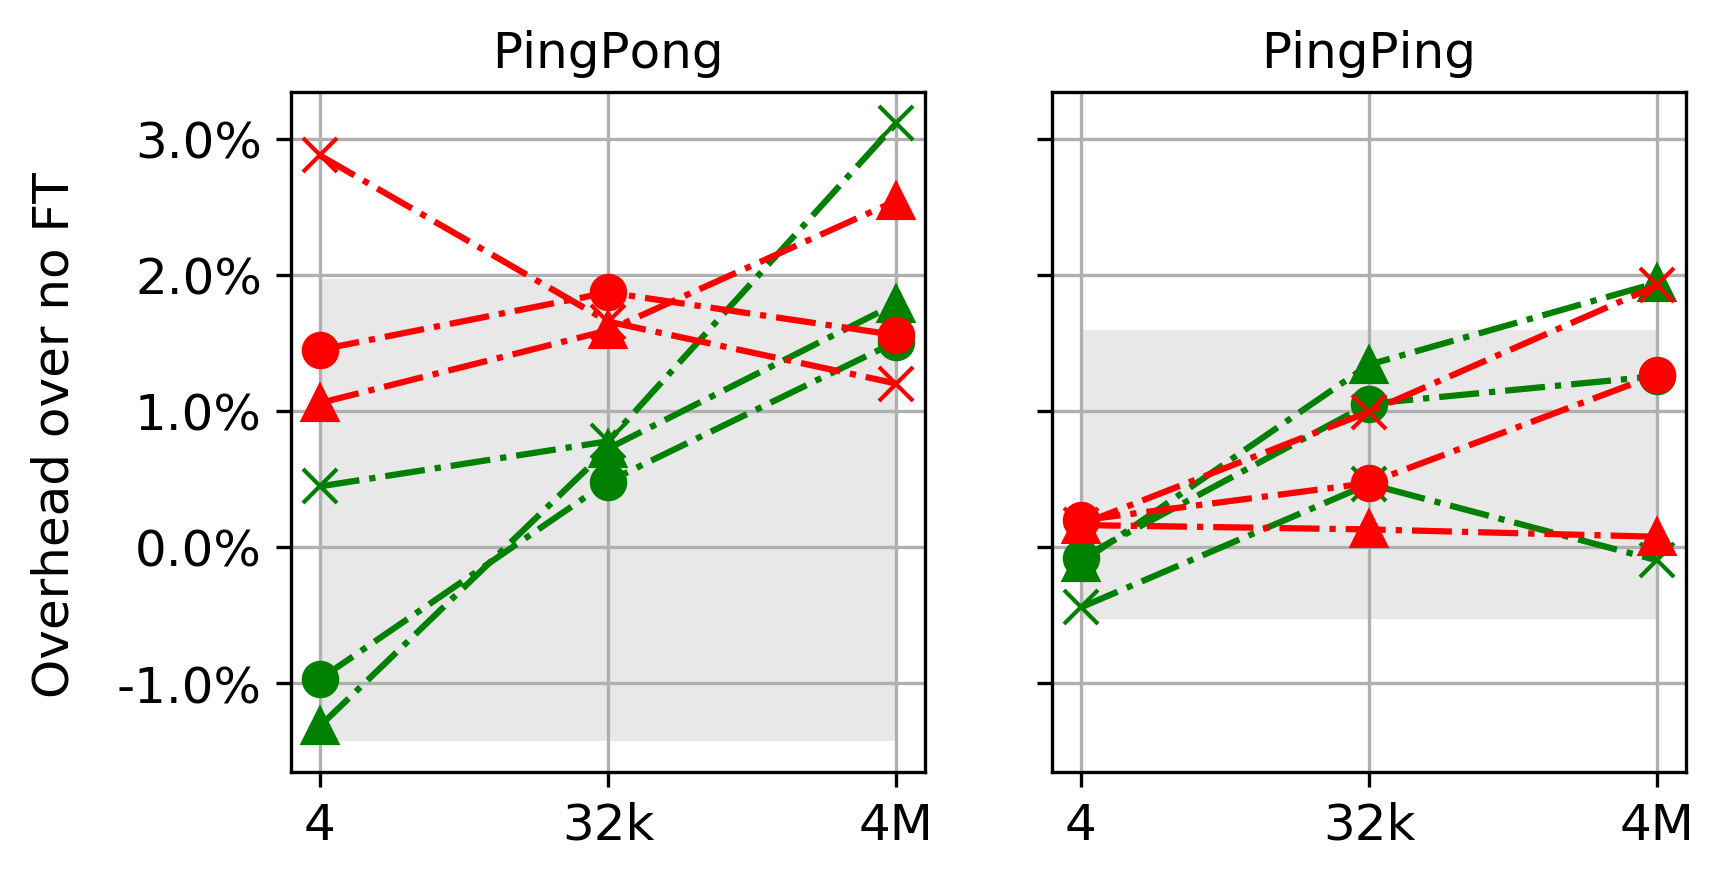
\includegraphics[width=\linewidth]{multi_pingping_pingpong_overhead.png}
  \label{fig:Ring}
\end{minipage}%
\begin{minipage}{.62\textwidth}
  \centering
  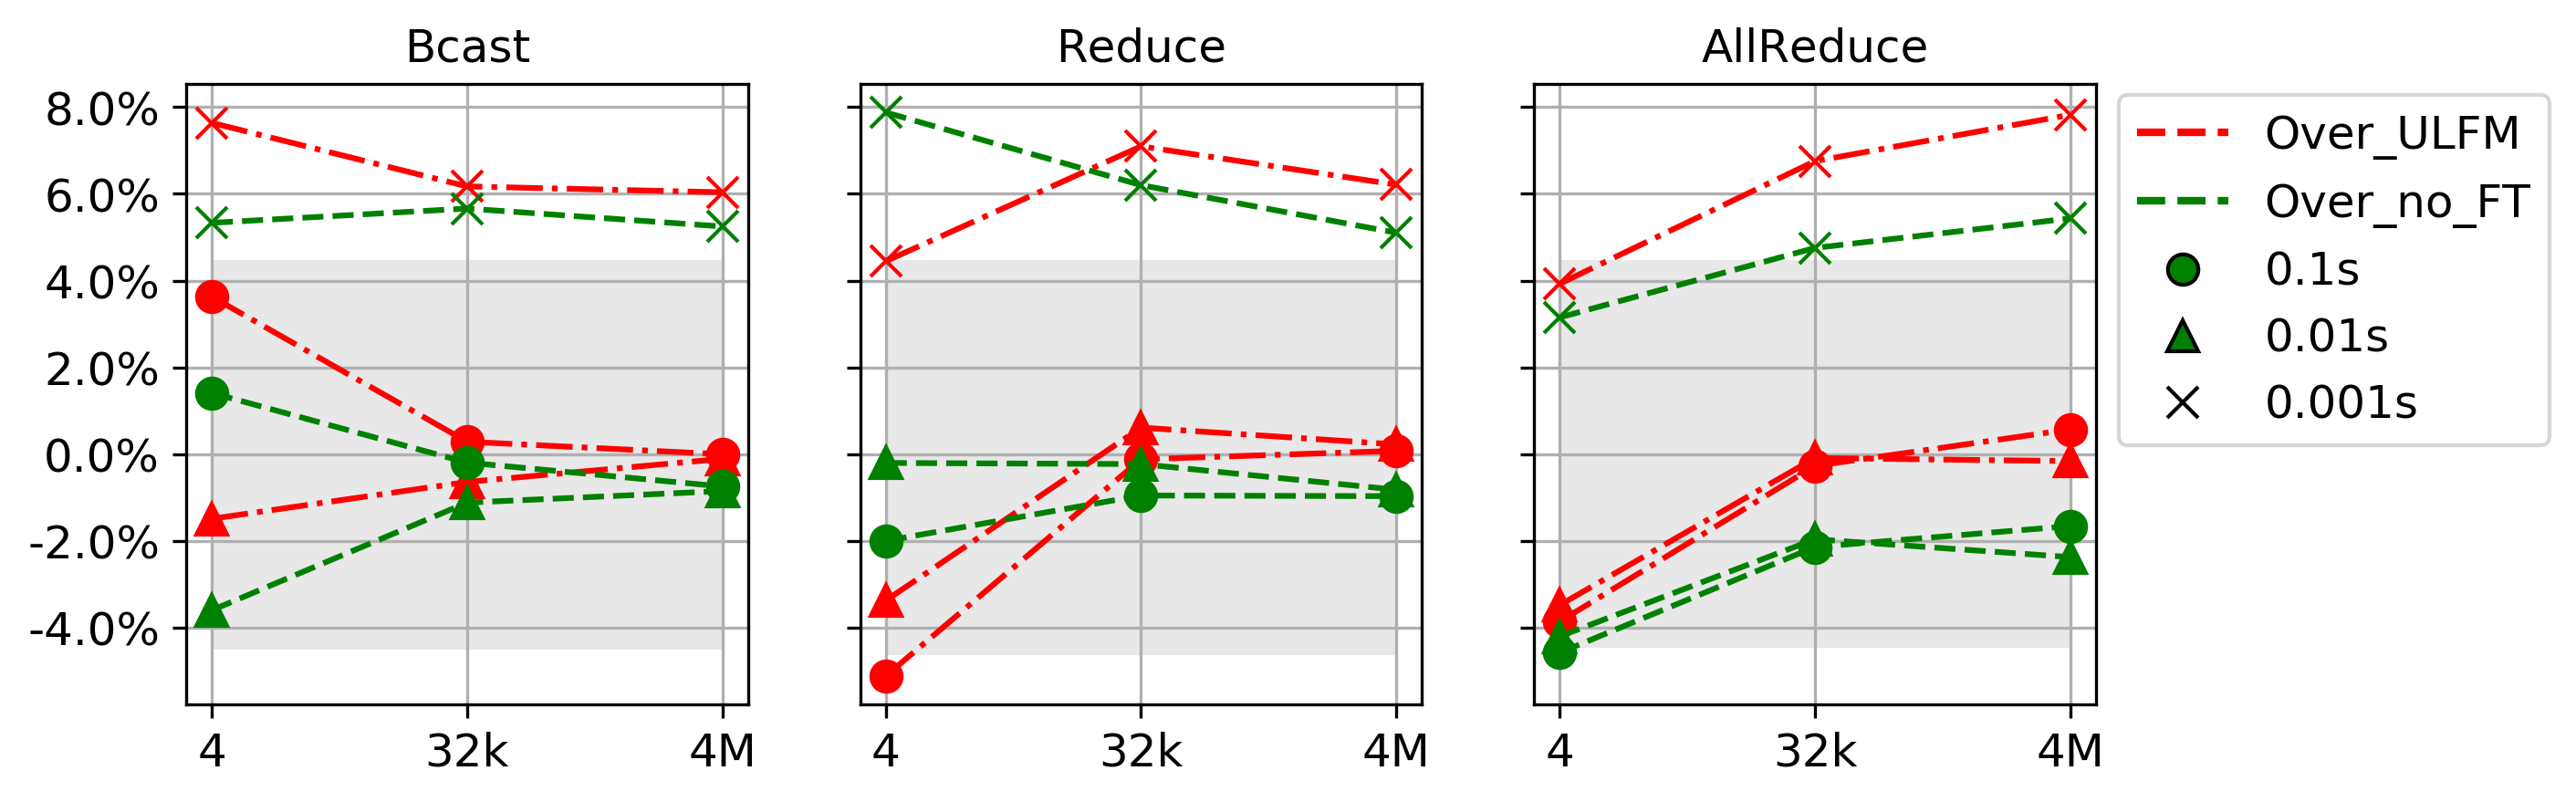
\includegraphics[width=\linewidth]{Bcast_overhead_with_ulfm_max_col.png}
  \label{fig:Reconnect Ring}
\end{minipage}
\captionof{figure}{PRRTE with fault tolerance overhead over PRRTE and ULFM using IMB}
\end{figure*}

Figure 7 shows the overhead incurred with P2P and collective communications, test results come from Intel MPI benchmark(v2019.2). All IMB-MPI1 suits can be successfully conducted with no false detection with $ \delta \geq 1 ms $. For the P2P setting, we run the benchmark on two nodes will all cores included using the "multi" option, which pairs core from both node as groups to ensure that no matter how daemon are binded the communication will be affected. For the collective we run the benchmark on 64 nodes using all cores. Any single test we using message size from several bytes to mega bytes, for each message size test last more than 20 second to ensure enough heartbeats emissions are occurred during the experiments. The PRRTE overhead is calculated by: latency of the benchmark suits with enable failure detection compared to disable failure detection. From the figure we can see that the latency of performance and bandwidth performance are barely affected by heartbeat periods from milliseconds to seconds. Notably, point to point communication overhead of all tested heartbeat values are less than three percentage. As for collective communication (Bcast Reduce and Allreduce) the overhead are less than eight percentage compared to a deviation of four percentage of the benchmark itself. Also we calculated the overhead compared to OpenMPI/ULFM2, shows that the overhead results are similar for P2P and collective respectively for all message size.

\subsection{Comparison with SWIM}
This section compares our failure detector with SWIM\cite{Abhinandan02}, using a random-probing based failure detection protocol and disseminates membership updates via network multi-cast. SWIM using subgroups to probe to decrease the randomness increases the scalability. To avoid false detection, SWIM uses suspicion mechanism, when a node does not reply direct or indirect probing in time, the initiator then judges this node as suspicious instead of failure, then broadcast
\begin{figure}[h]
  \centering
  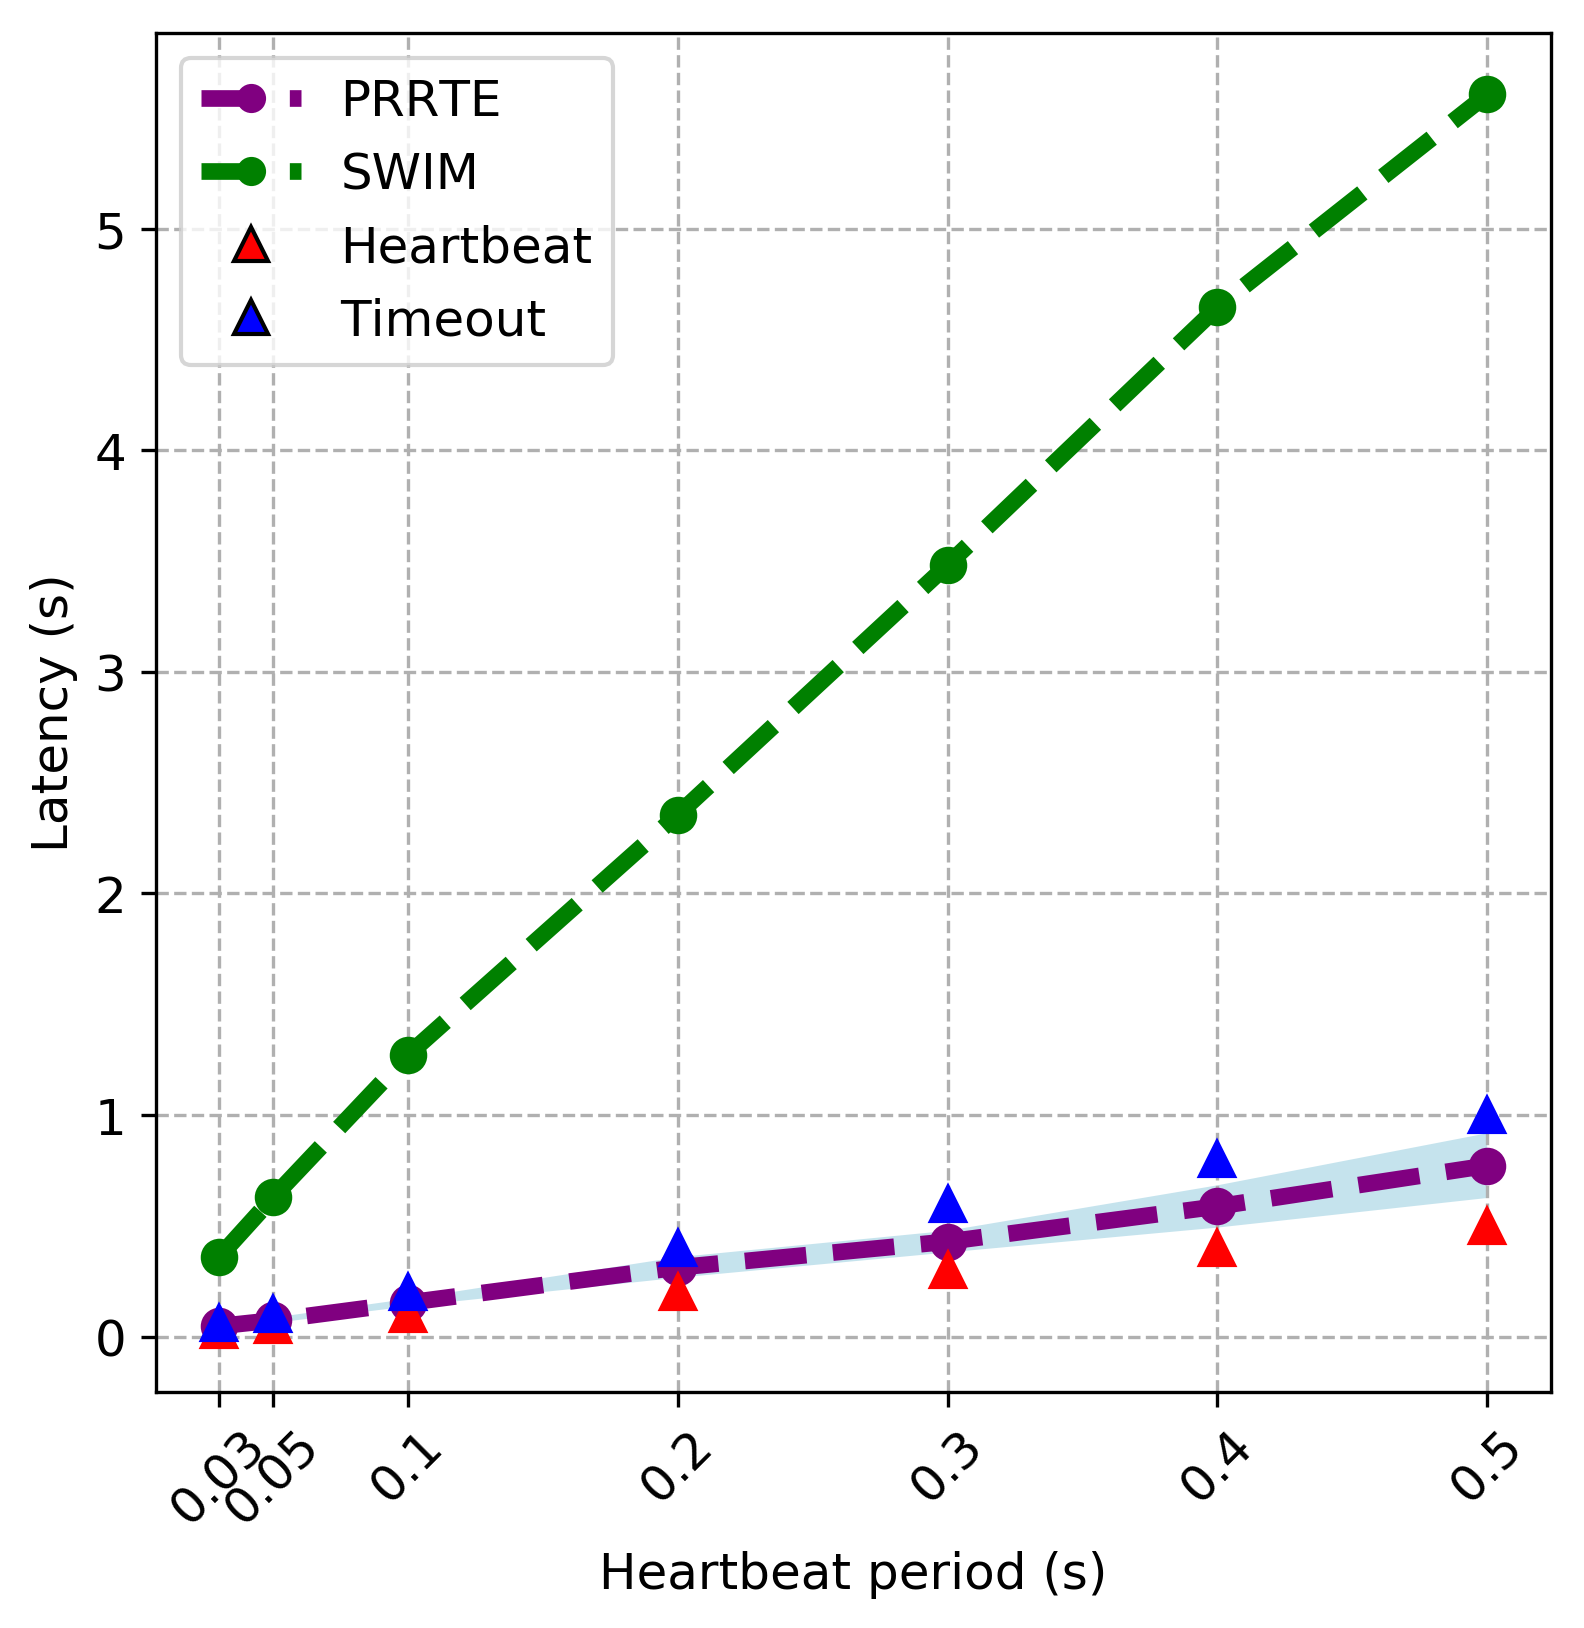
\includegraphics[width=\linewidth]{HB_prrte_swim.png}
  \caption{Detection and Propagation delay compared to SWIM using Go-Memberlist}
\end{figure}
this suspicious info in the subgroup, if any node in the subgroup receives an acknowledge before the timeout, it will unmask the suspected node as alive, otherwise mark as failure. In order to improve the efficiency of multi-cast, SWIM use a infection-style dissemination mechanism as information spreads in a manner analogous to the spread of gossip in society, or epidemic in the general population.

Figure 8 compares detection and propagation delay between our PRRTE detector and SWIM detector of node failure. For the SWIM implementation, we use Go-Memberlist (\#a8f83c6) which is integrated with Go instead of mpi, however we use go-mpi binding to enable SWIM run as mpi application, we use mpi barrier to synchronize before injecting failures in SWIM, and SWIM reports failure through Go-Memberlist callback functions. We run all Memberlist tests only up to 256 processes which is the upper bound of SWIM member limited by maximum connection requests on Transmission Control Protocol (TCP) socket, however this implementation suffers from connection storm and cause consequently crash of continuous running. 

For PRRTE, we also synchronize with barrier, and use our benchmark to inject node failure, detection and notification latency are collected on each process. We run all tests up to 768 processes on 64 nodes.We compare the latency of detection and propagation with different heartbeat period value, for all test we set the timeout equal two times of heartbeat. We can clearly see that for PRRTE the detection latency is around the middle of heartbeat and timeout, and the receive of notification happens immediately after the detection which shows the efficiency of our propagator. However for SWIM even with smaller number of processes the delay is still around 10 times of heartbeat period. The variation come from the randomness of when the node failure happened.

Figure 9 compare the scalability of the detector with regard to the number of deployed processes. We set the heartbeat period to 0.5 second with timeout of 1 second. For smaller number of processes PRRTE failure detector is stabilizing in approximately 0.75 second, because of the randomness of when the failure happened between two contiguous heartbeats, while the stabilization delay of SWIM is around ten times of heartbeat period. As the number of processes increases, PRRTE's latency remains almost the same. But SWIM shows a linear increase with will be the limitation of scaling up(with the assumption it can solve the maximum connection requests limit). For PRRTE with 4K processes the stabilization is still between heart period and timeout.

\begin{figure}[h]
  \centering
  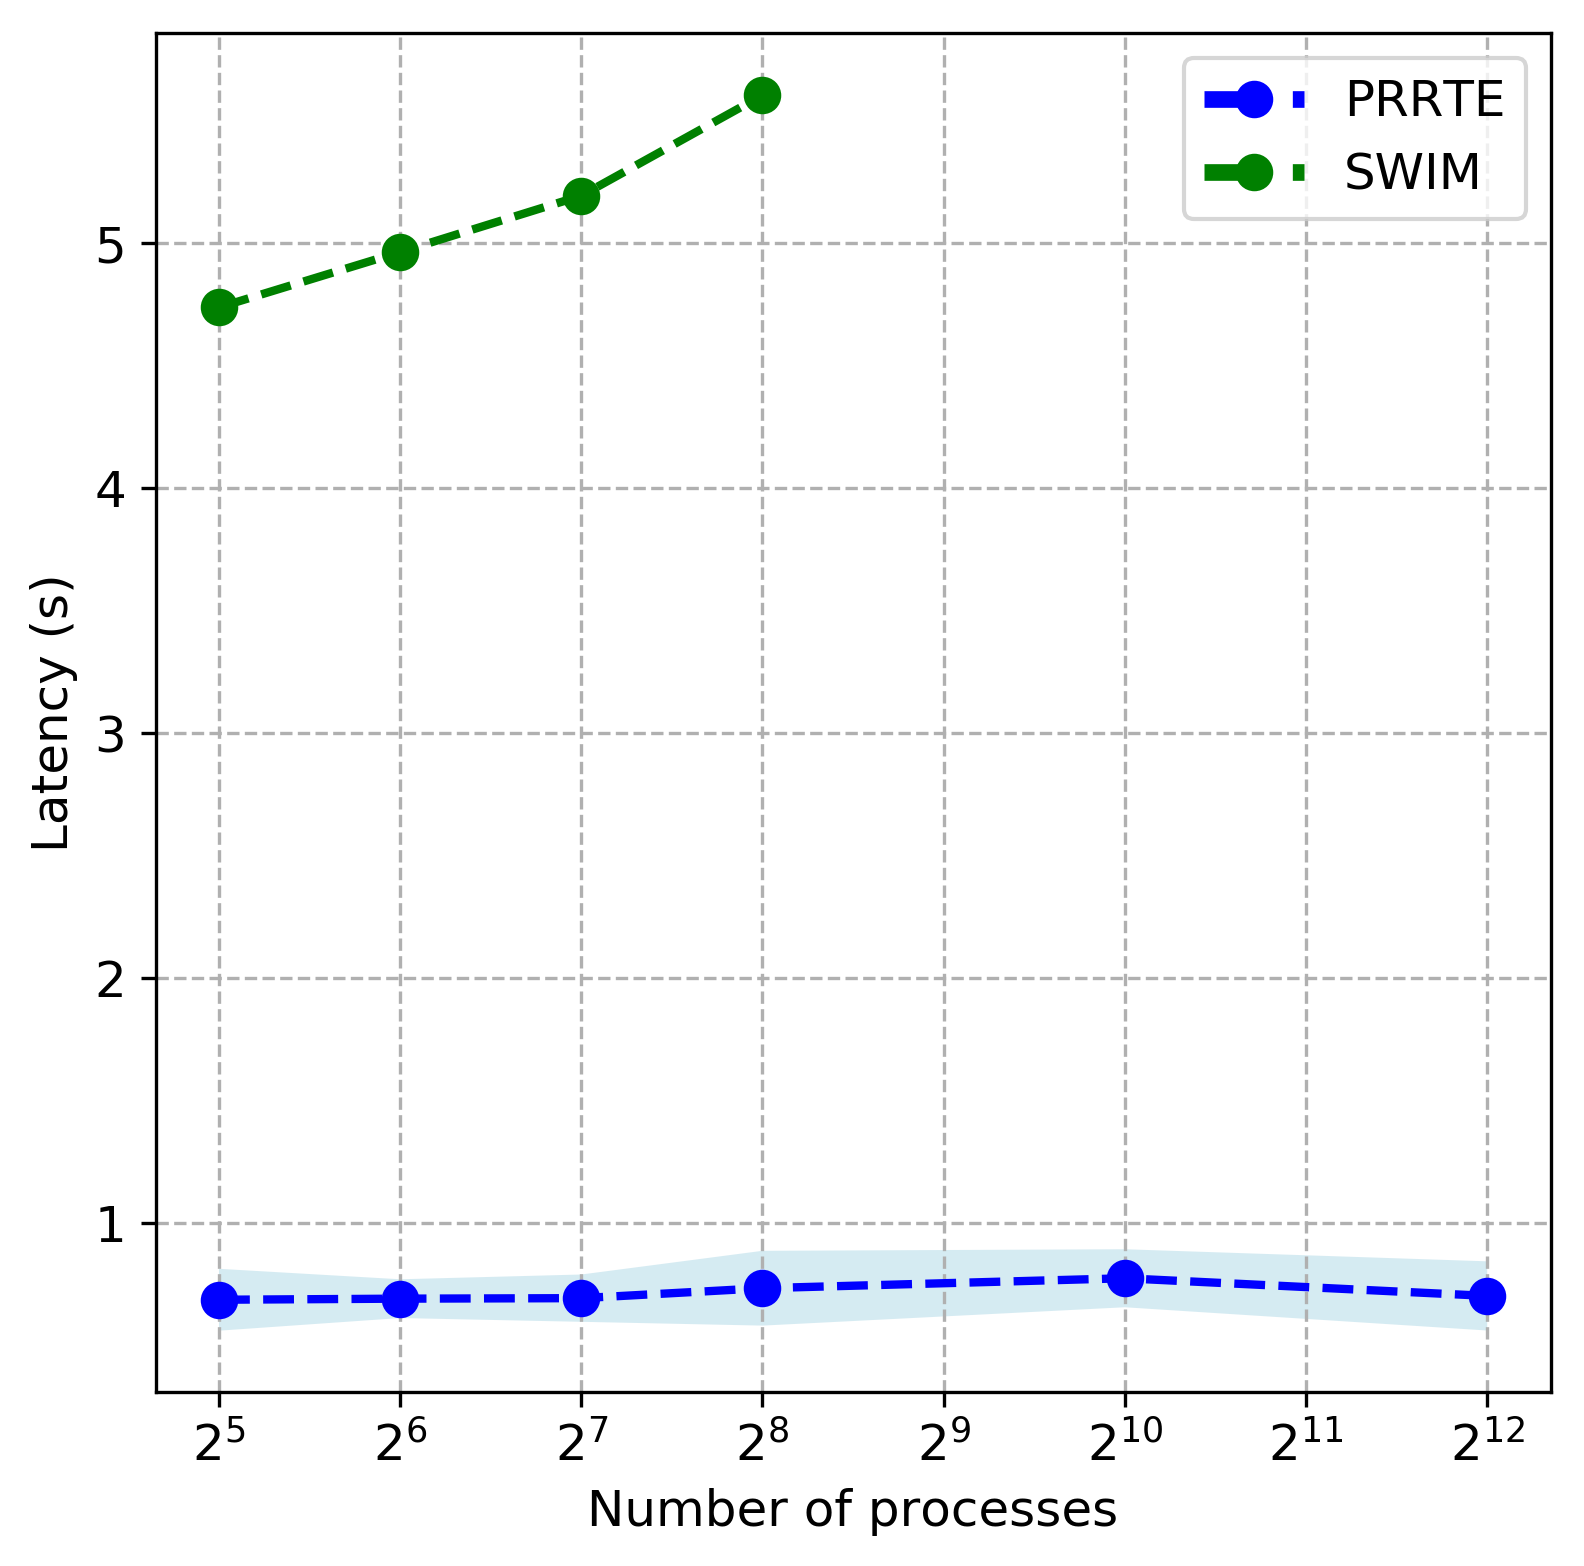
\includegraphics[width=\linewidth]{Scale_prrte_swim.png}
  \caption{Scalability compared to SWIM using Go-Memberlist}
\end{figure}

\subsection{Comparison with ULFM for process failure}
This section compares our failure detector with our previous work ULFM\cite{George18}, the ULFM implementation also has two main components: process level detection ring, and propagation overlay with all launched processes. The detection ring is built at Byte Transfer Layer (BTL) level - which provides the portable low-level transport abstraction in OPEN MPI. The current detection implementation provides several mechanisms to ensure the timely activation and delivery of heartbeats:
\begin{enumerate}
  \item using a separate, library internal thread to send the heartbeats in order to be separated from the application's communication, this also avoid the possible heartbeat delay of compute intensive application. For receiver it need to poll BTL engine to check the aliveness of its successor. 
  \item using RDMA put to raise a flag in the receiver's registered memory, by using the hardware accelerated put operations solves the problem of active polling BTL engine. 
  \item ULFM is also using in-band detection for process to report unreachable error directly to the propagator.
\end{enumerate}

The propagation overlay is also built at BTL level, the small message size of propagation information contains a callback function index which ensures that the received process states update information can be analyzed by upon reception. This method provides independence from the MPI semantic (including matching), however the overlay is constructed with all processes, which means that all participated process need to paopagate/forward the error information, also the lower bound of reaching any process is bounded by $\log_2(Number of Processes)$.  

However, PRRTE process failure detection is implemented in a much simpler mechanism, the daemons are monitoring the lifeline of all local processes, this mechanism doesn't bring any pressure to the applications' communication resources, also don't need RDMA hardware accelerate support. For the propagation of PRRTE, the overlay is built at daemon level which highly decreases the participates, with less participates the total messages transferred and forwarded is much less than the case of ULFM, also the lower bound is $\log_2({Number of Nodes})$. With the development of more powerful multi-core nodes, the benefit of node level propagation will be much more significant.

\begin{figure}[h]
  \centering
  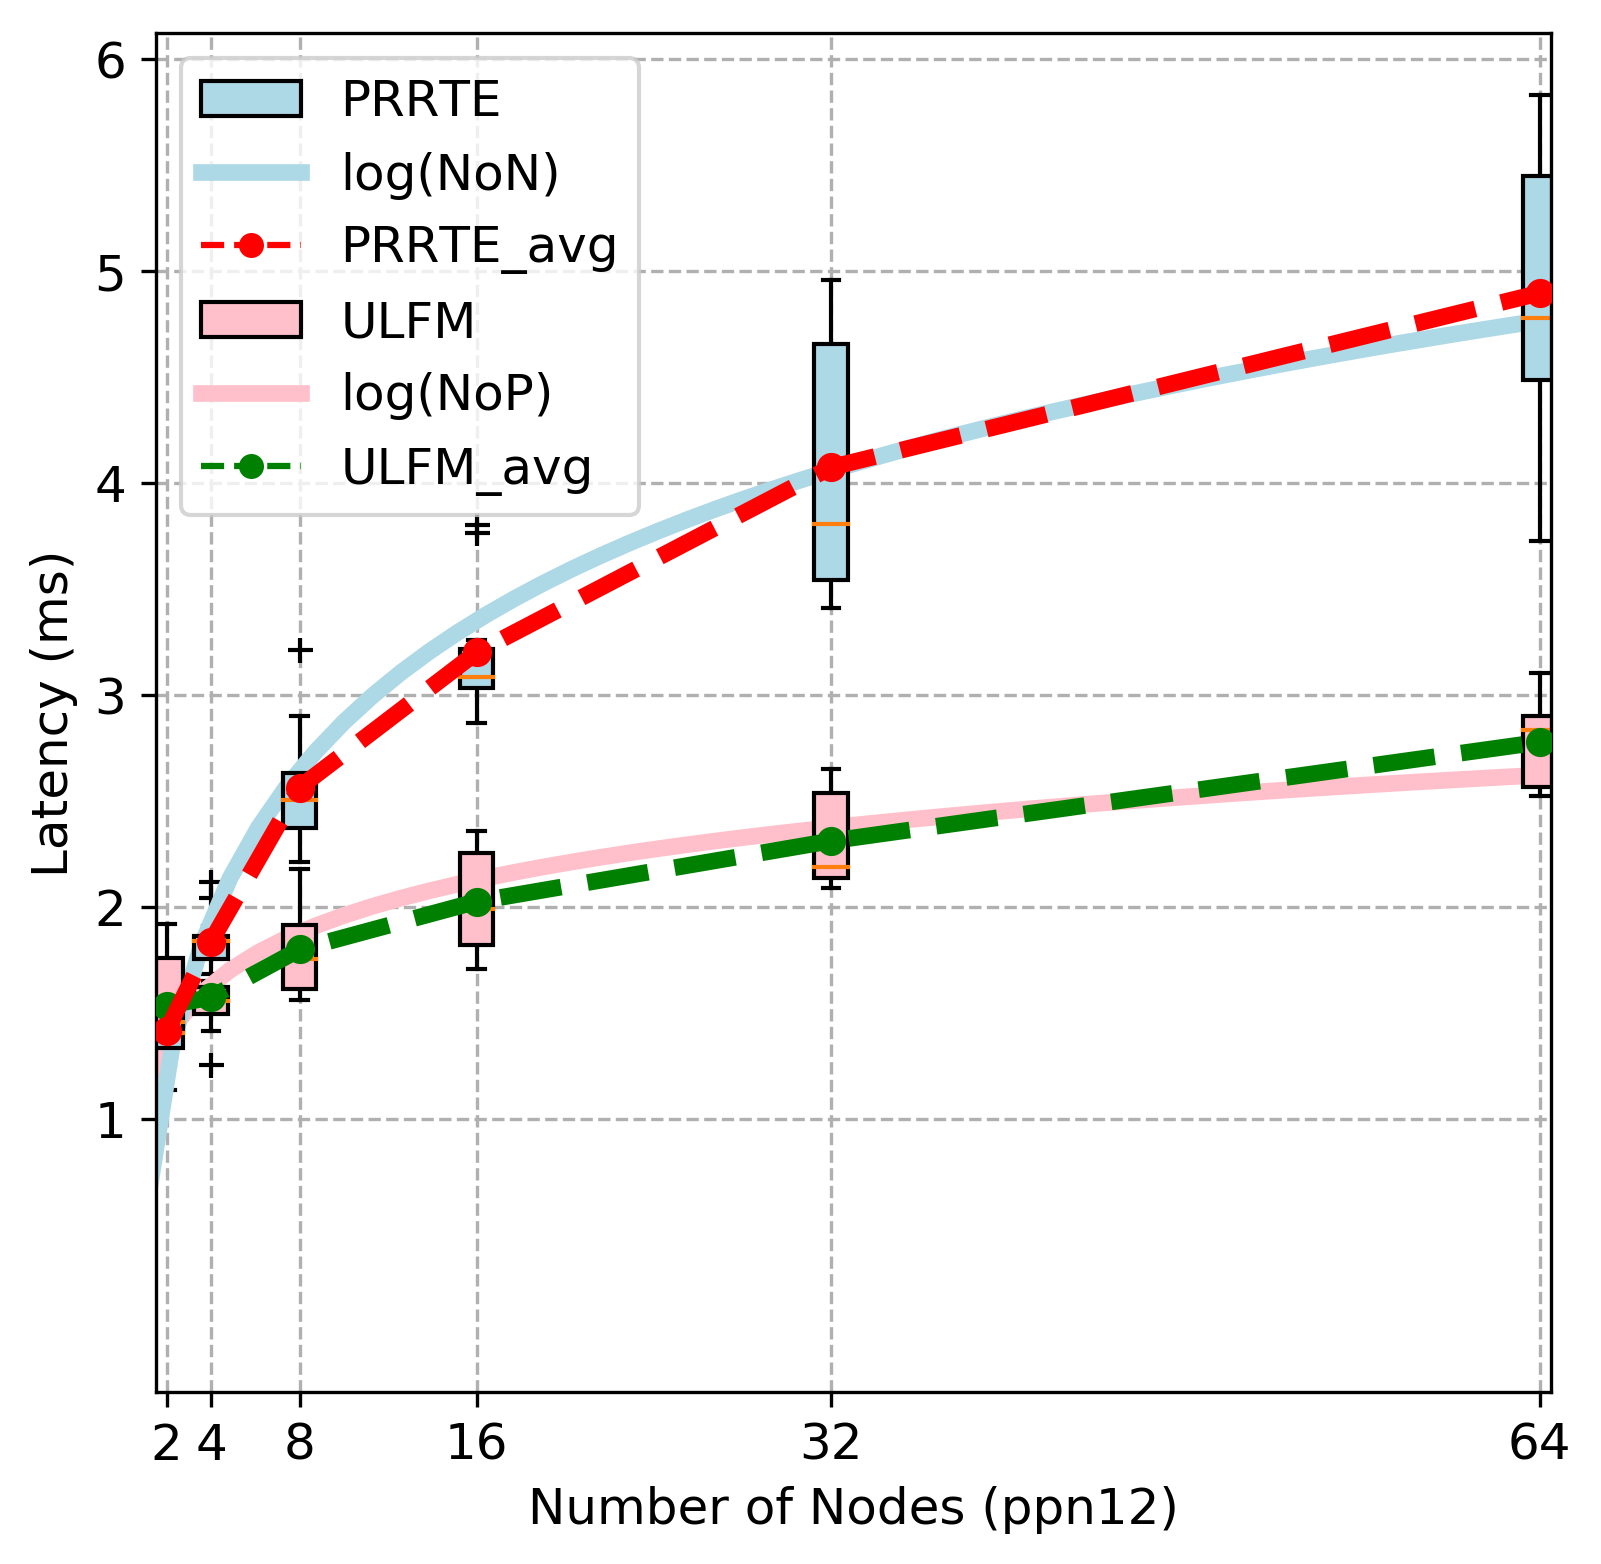
\includegraphics[width=\linewidth]{Process_Failure_log_fit.png}
  \caption{Process failure detection and propagation delay compared to ULFM}
\end{figure}

Figure 10 compares the latency of process failure detection and propagation of ULFM and PRRTE. The sensitivity of ULFM heartbeat without false detection is 10 milliseconds, but we want to compare the best performance from ULFM using high speed in-band detection which is faster than using the lowest heartbeat period. For PRRTE the daemons in charge of detecting any process failure. PRRTE is using TCP to broadcast among daemons, each daemon using the PMIx notification method to distribute the error information to all hosted processes. The experiments are conducted on our local cluster NaCl from 2 nodes to 64 nodes using all cores on each node, all processes are equalled mapped to node and bind to core, by doing this ULFM can use the in-band shared communication for detection and propagation. We can see with a simpler implementation, PRRTE still shows the detection and propagation time is less than 5 millisecond with different number of nodes start from 2 to 64 using TCP. For ULFM the detection and propagation delay increase from 2 millisecond to 3 millisecond as the processes number increases with number of nodes using infiniband. For both PRRTE and ULFM the latency increase trend fit to $ a*\log_2(N) + b $, which can be easily scale up to hundreds of thousands of nodes. Similar result shows in figure 11 from Cori with more processes on each node, we can see that with 4K processes the detection and propagation latency is about 10 milliseconds. This result vindicates the efficiency of our broadcast and propagation algorithm.  

\begin{figure}[h]
  \centering
  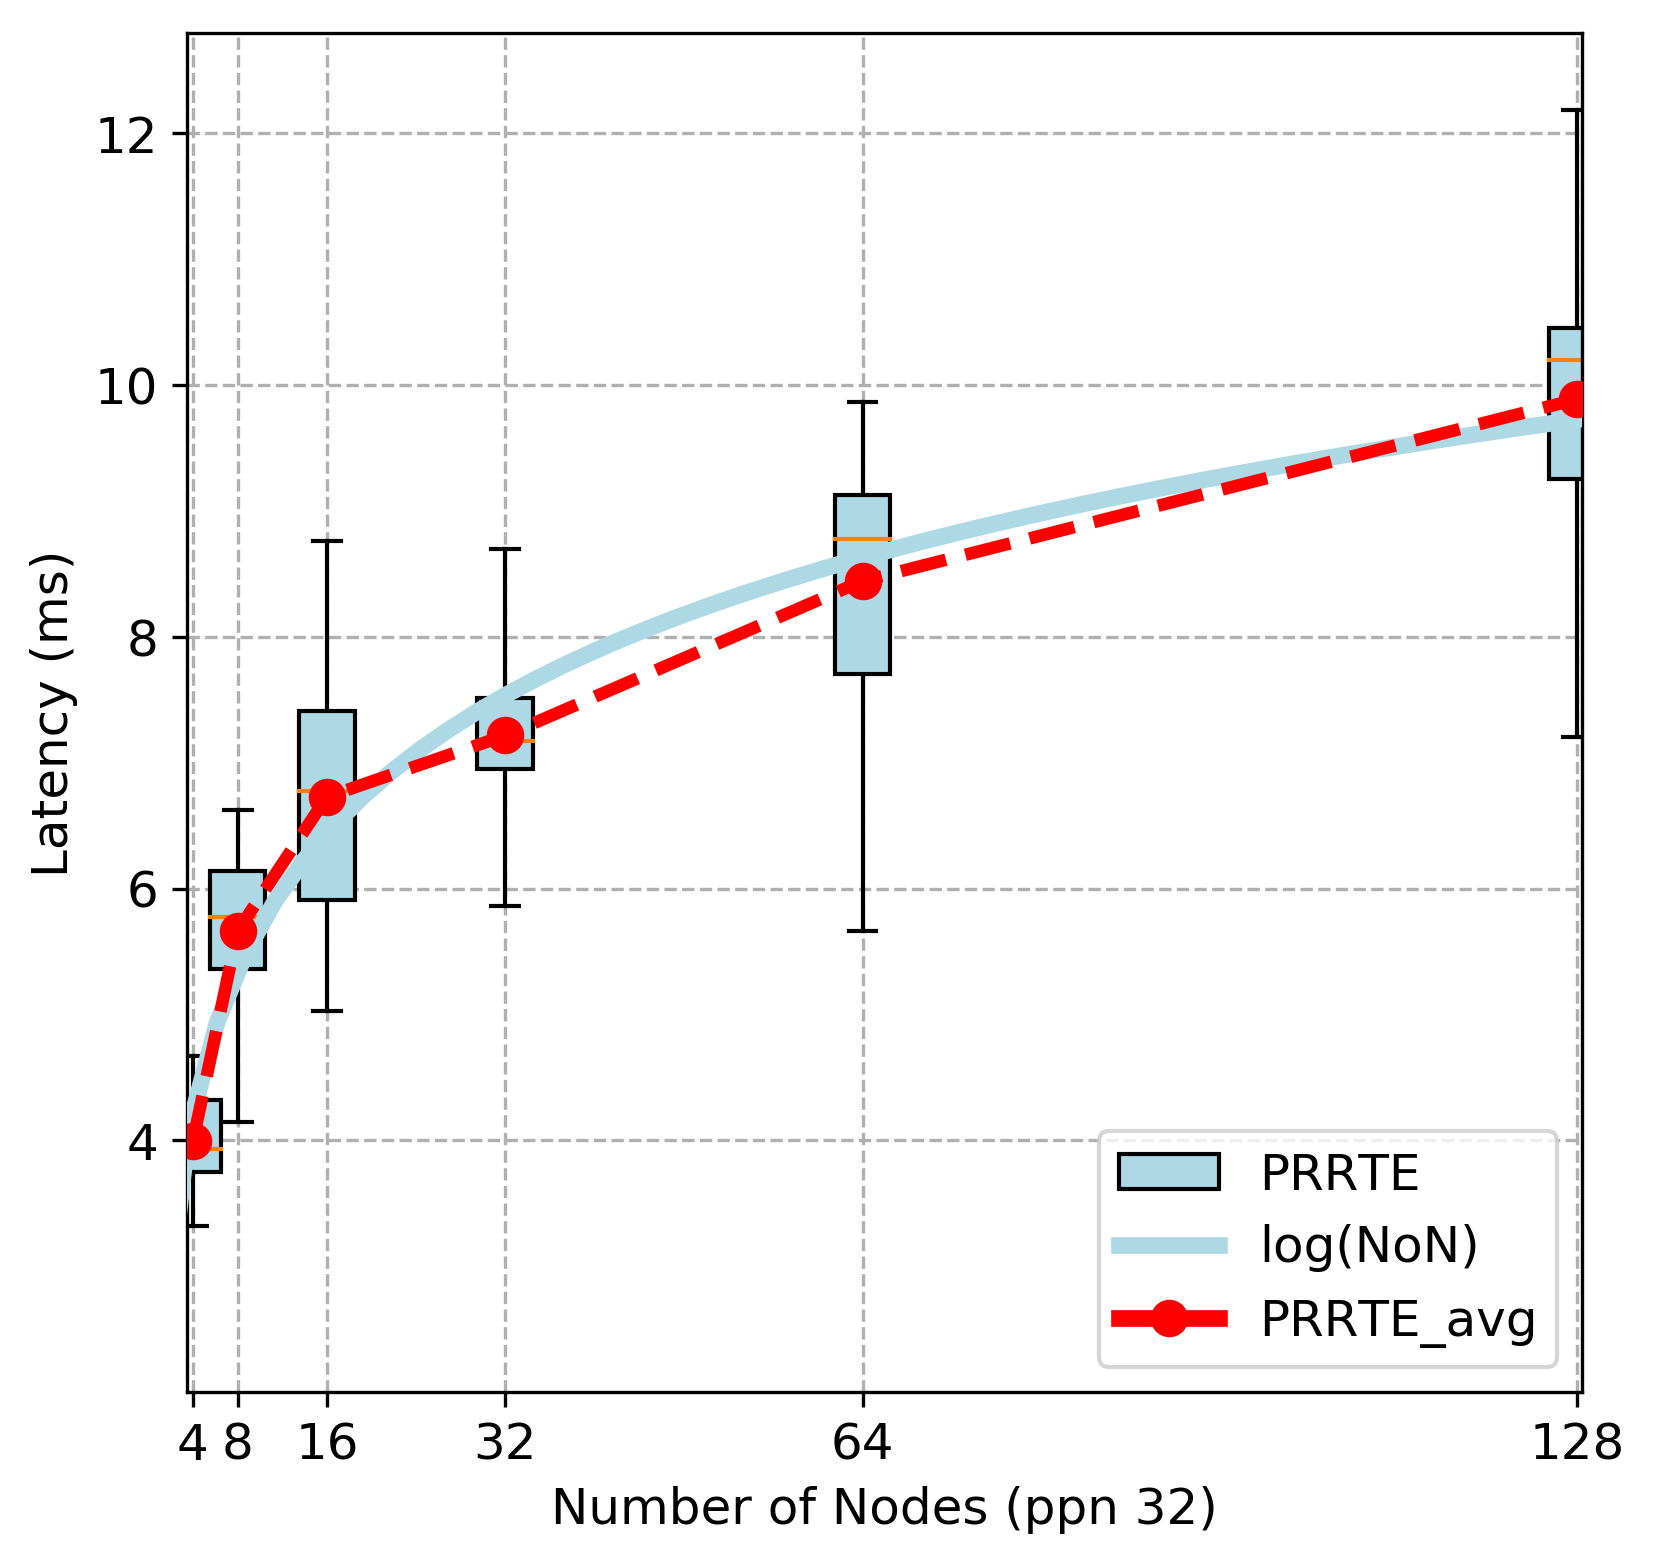
\includegraphics[width=\linewidth]{Cori_Process_Failure_fit.png}
  \caption{Process failure detection and propagation delay on Cori}
\end{figure}

\subsection{Node failure detection}
Future more, we want to explore the performance of our heartbeat detector  for node failure detection and propagation from two perspectives. 
\begin{enumerate}
  \item Latency of detection time and propagation time with different heartbeat periods.
  \item The detection and propagation efficient using fixed heartbeat and timeout period but with different number of nodes.
  \item Detection latency of multiple node failure.
\end{enumerate}

\begin{figure}[h]
  \centering
  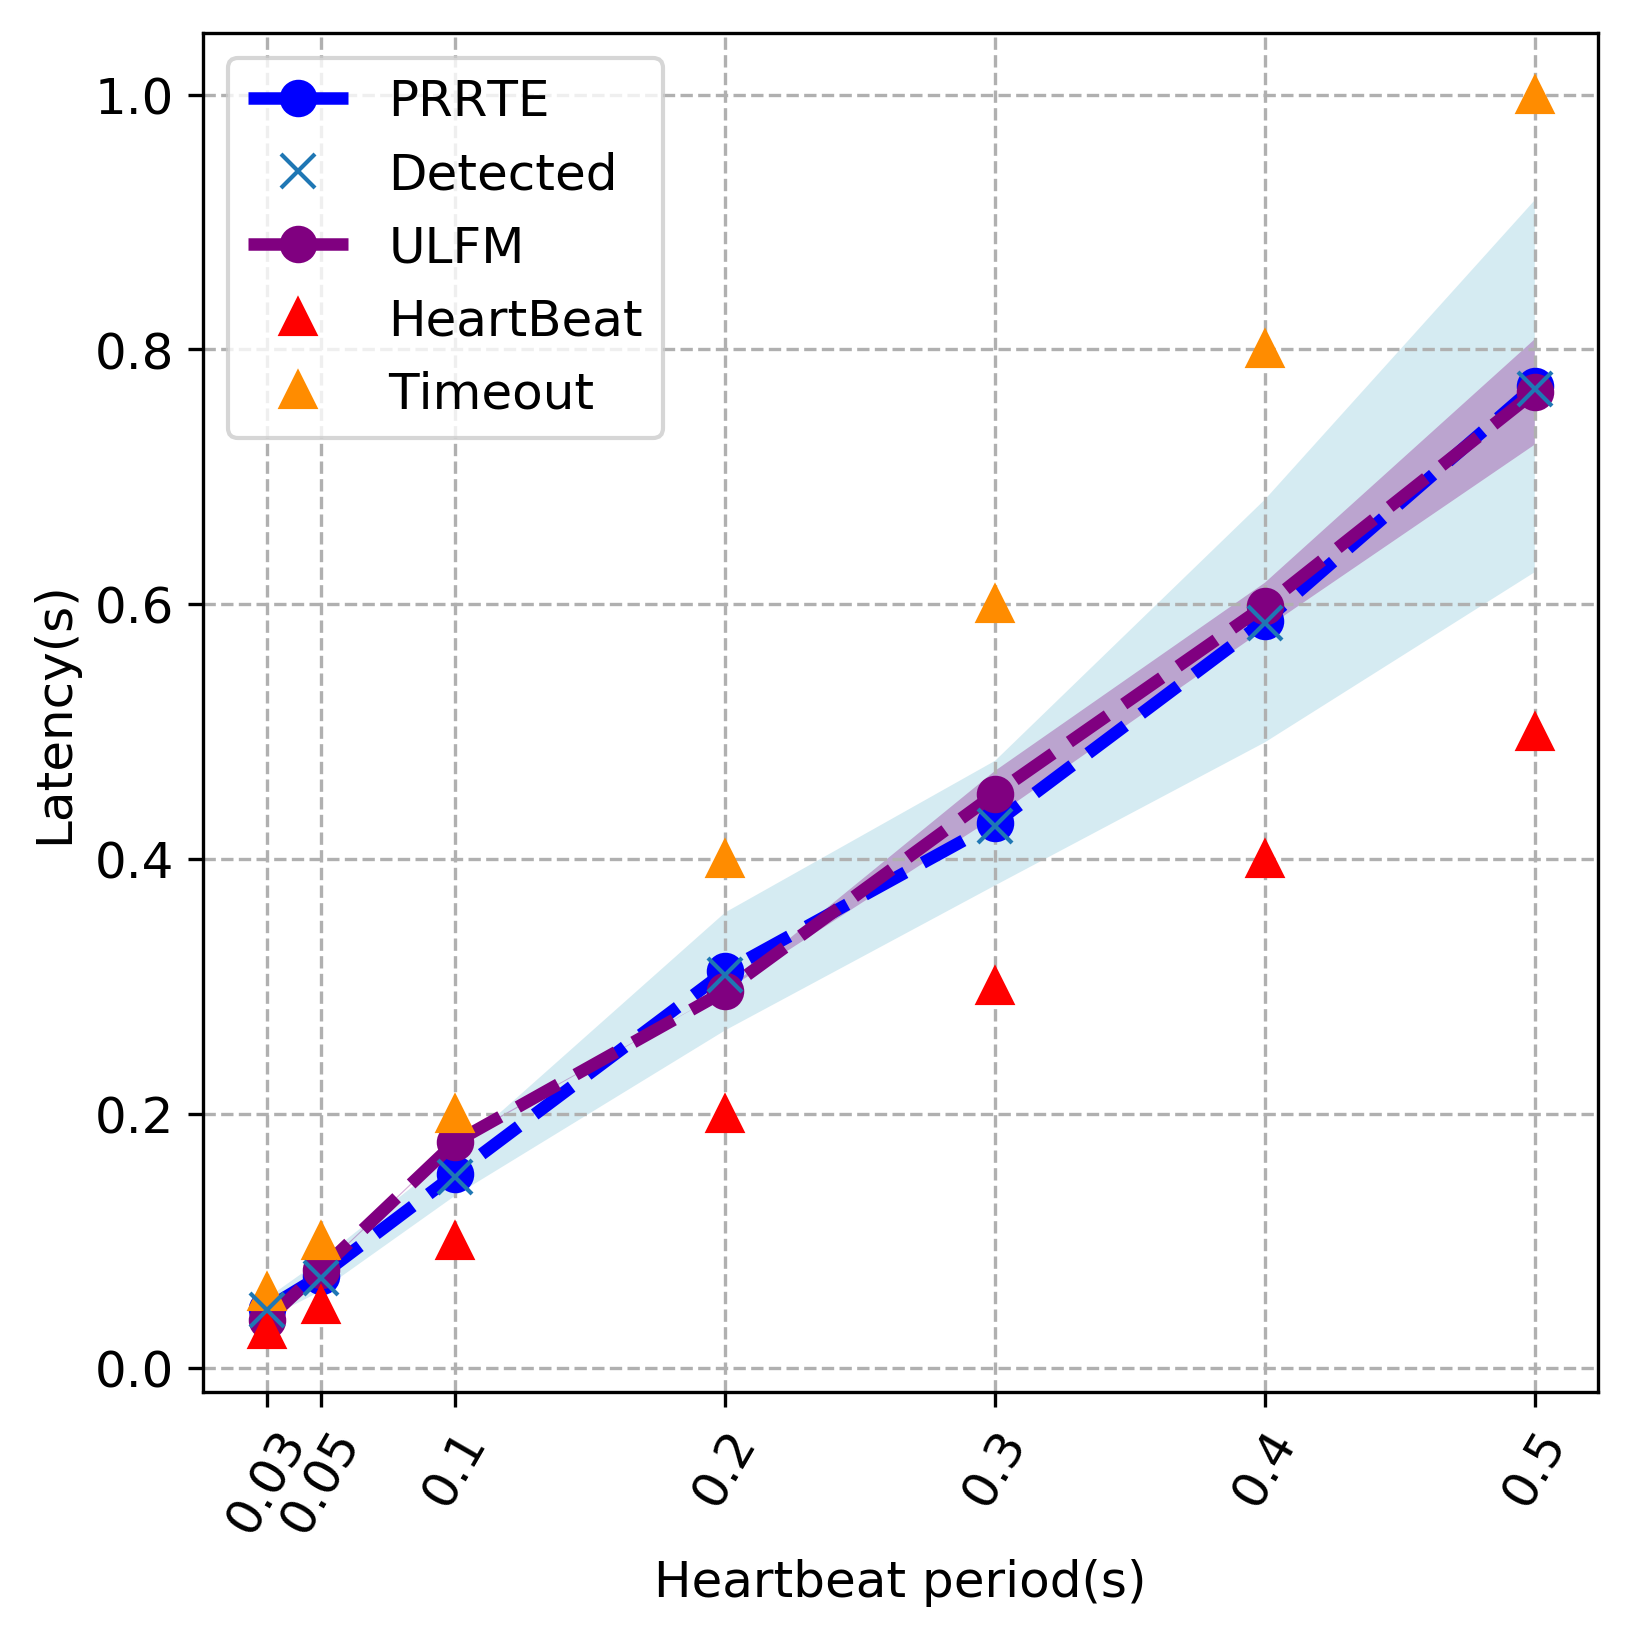
\includegraphics[width=\linewidth]{PRRTE_ULFM_new_nodebug.png}
  \caption{Daemon Failure detection and propagation delay compared to ULFM with different heartbeat period}
\end{figure}

Figure 12 presents the behavior observed when injecting single daemon failure under different heartbeat period setting. We conducted the experiments on 64 nodes with 764 processes. For PRRTE after synchronizing, we inject a node crash by choosing a process to kill its host using the parent process identifier. However, ULFM doesn't have capability of detecting node failure, we simulate "node crash" by kill the last process on that node. With the process ring detector this particular process failure will be detected by its observer on another node, this behavior is the same as PRRTE node to detect node failure. Also we assume that the time different between the daemon failure and process failure is trivial which is confirmed later in the experiment. For the heartbeat period setting we starts at 30 millisecond to half second for both PRRTE and ULFM. For all heartbeat periods we set $ \eta = \delta * 2 $. From the figure we can see that the latency for all cases are bound by $ (\eta - \delta,\eta) $.

Figure 13 shows single node failure detection and propagation performance with fixed heartbeat period $ \delta = 0.5s $ tested with different number of nodes. Once the node is failed all processes hosted on that node will be affected, the 
observer node will fetch and pack the information of all affected processes then distribute the packed message once.
\textbf{
\begin{figure}[h]
  \centering
  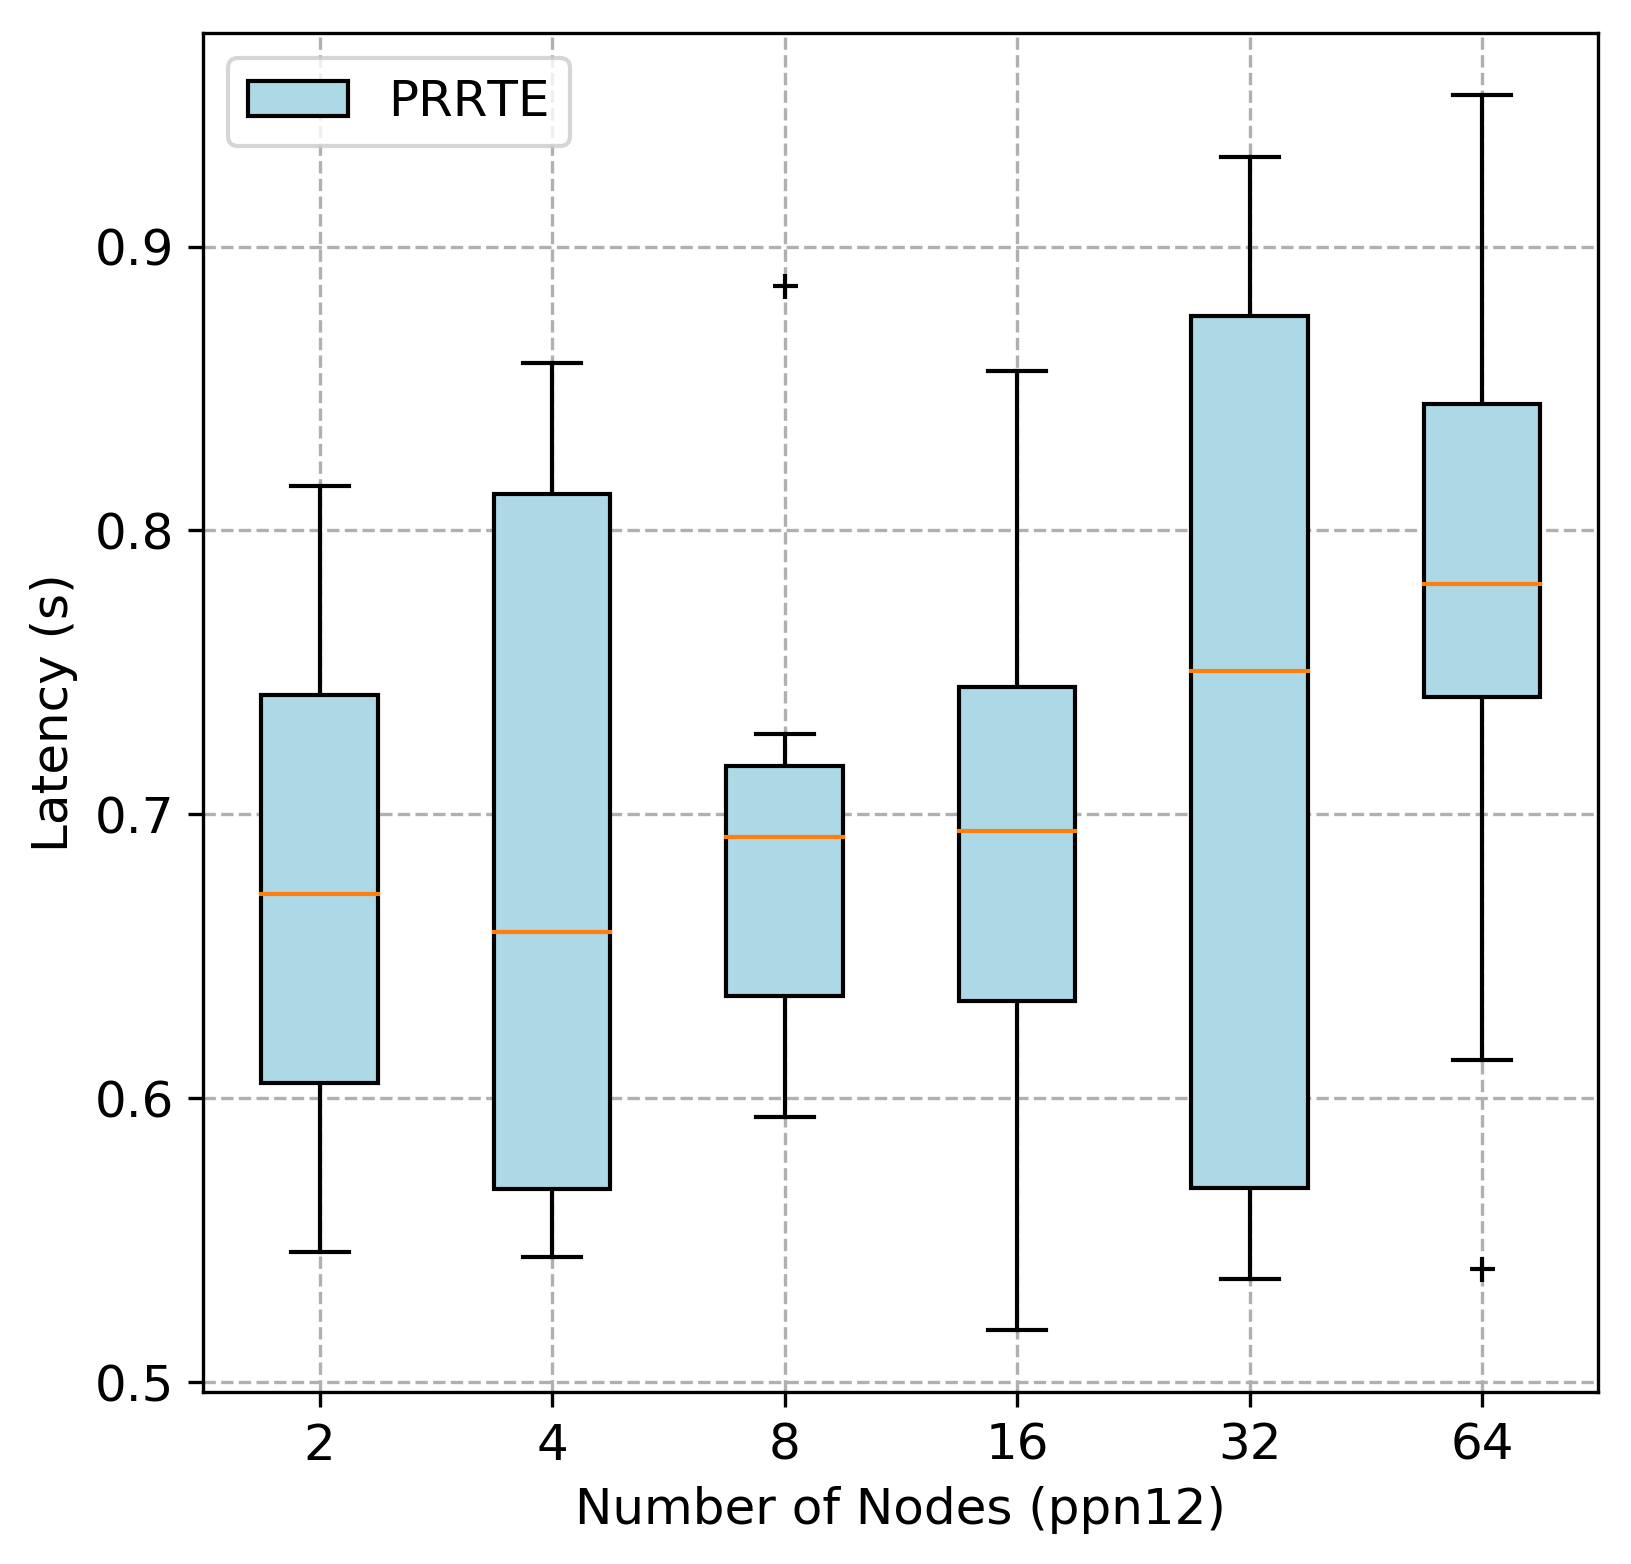
\includegraphics[width=\linewidth]{Daemon_prrte_only.png}
  \caption{Daemon Failure Detection and Propagation delay with different number of nodes}
\end{figure}}
However, for ULFM all affected processes need be detected by their observers independently, this will suffer from the collisions on the reliable broadcast propagation. For the worst case, all affected processes are adjacent in the detection ring, for each affected process need to re-connect and update the ring, bring a linear increase of $ \eta $ to the detection latency. From the figure see that PRRTE can detect and propagate a node failure between (0.5s, 1s) for all tested number of node. 

The last experiment (Figure 14) investigates the effect of multiple node failures happened in the system. The test setting is the same as single node failure case, except we inject multiple node failures from children processes. For the first scenario, injecting failure to nonadjacent nodes, the detection and propagation are independently conducted by different observer nodes which is a parallel execution. And the results in the figure show that the latency is a constant value which is not affected by the number node failure. The worst scenario is to inject failure to contiguous N nodes, all failures are detected by a single observer (switches to observing the predecessor of the detected failed node). This shows a serial execution. For each node failure it will cause an extra delay of $ \eta $ to the detection latency of the following node failures. From the figure we can see the results matches a linear increase. This suggest that from fault tolerance perspective the system will be more stable and reliable by building the detection ring in a arbitrary layout of nodes, avoid choosing predecessor and successor from the same cabinet.  

\begin{figure}[h]
  \centering
  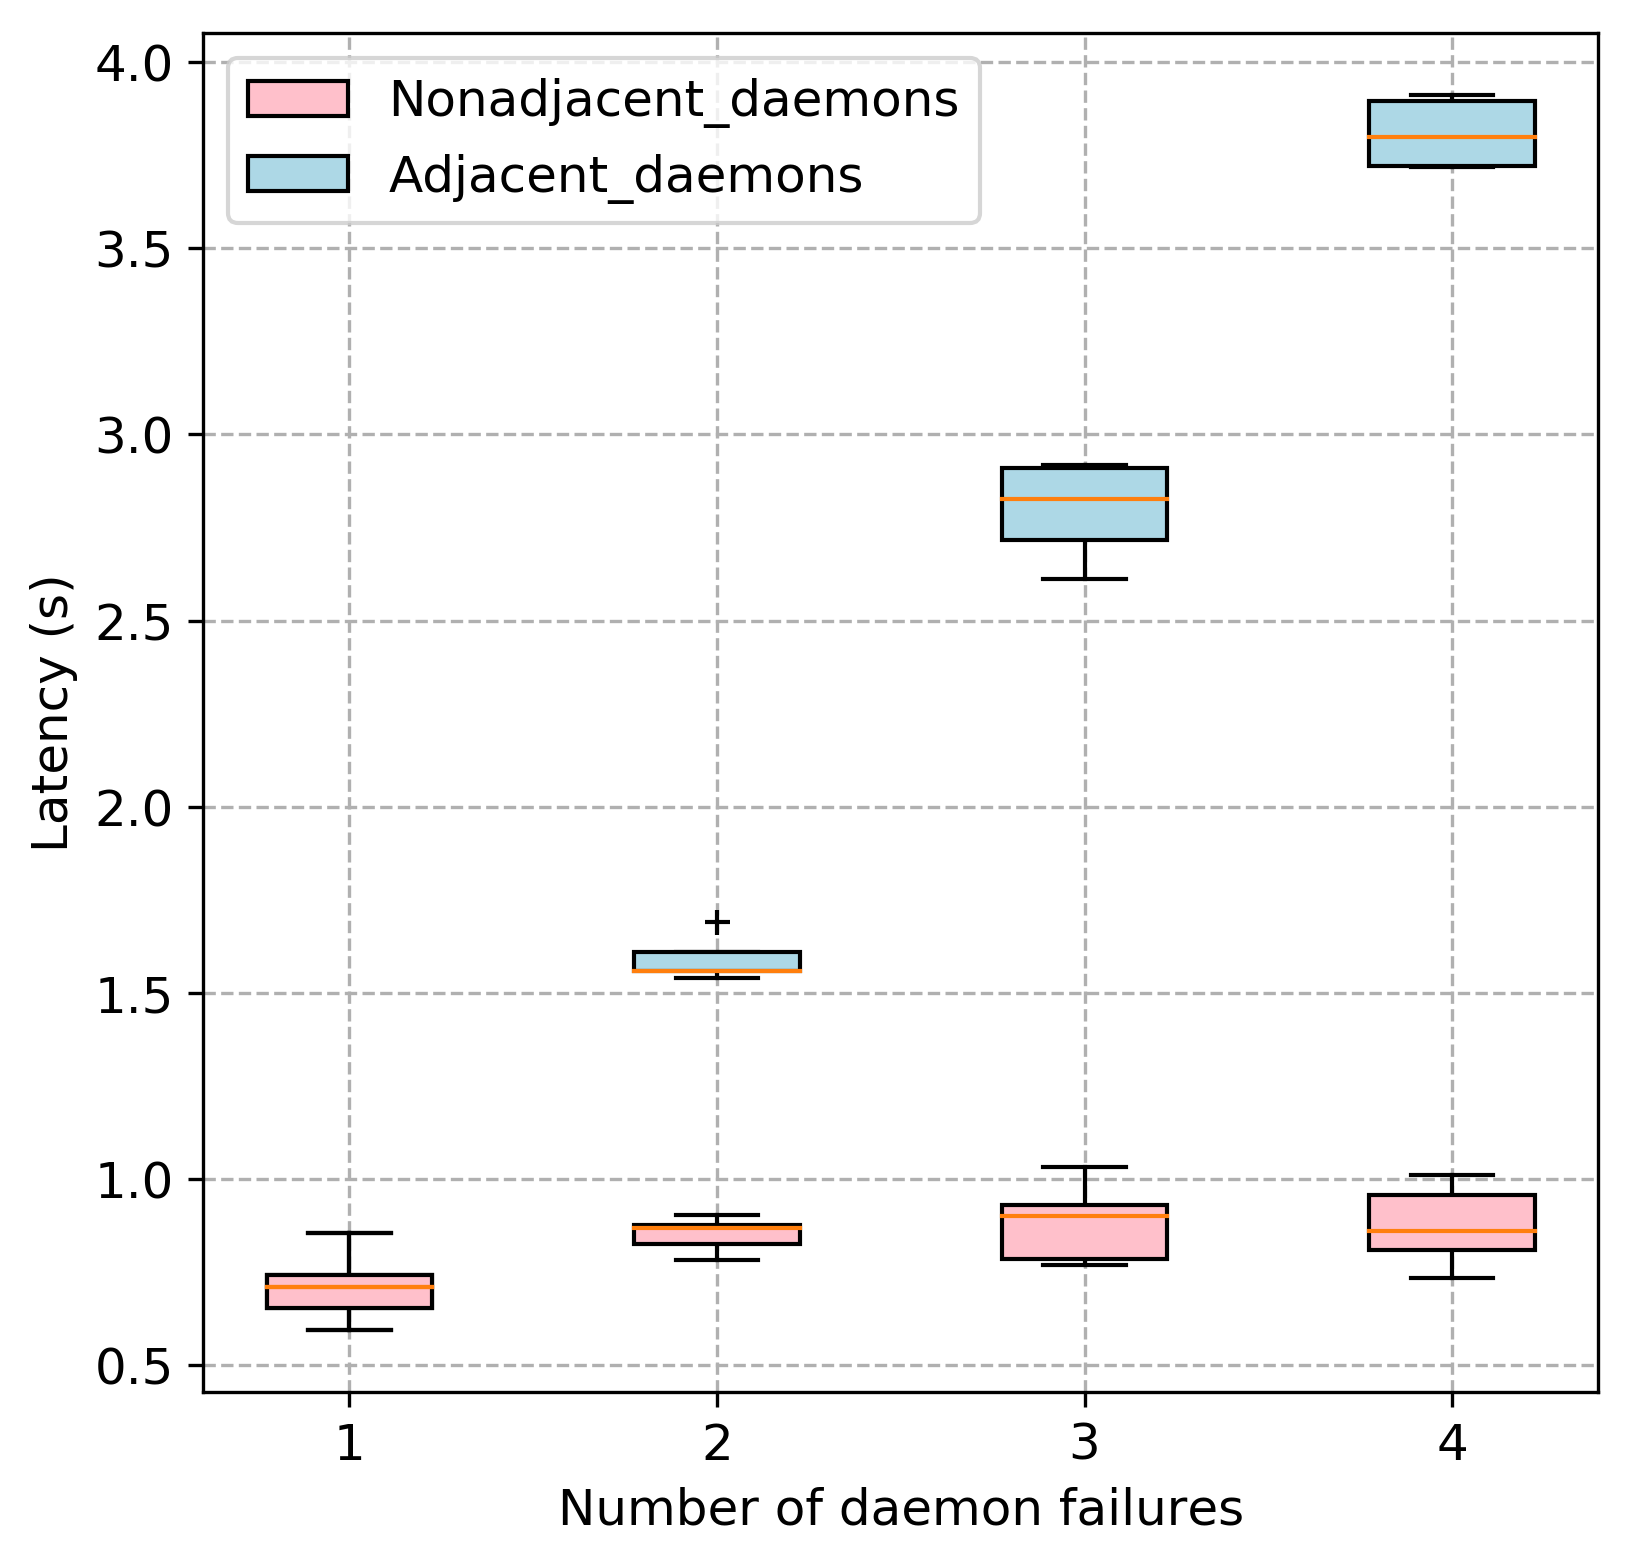
\includegraphics[width=\linewidth]{multi_daemon_failures.png}
  \caption{Multiple process failures at the same time}
\end{figure}

\begin{figure}[h]
  \centering
  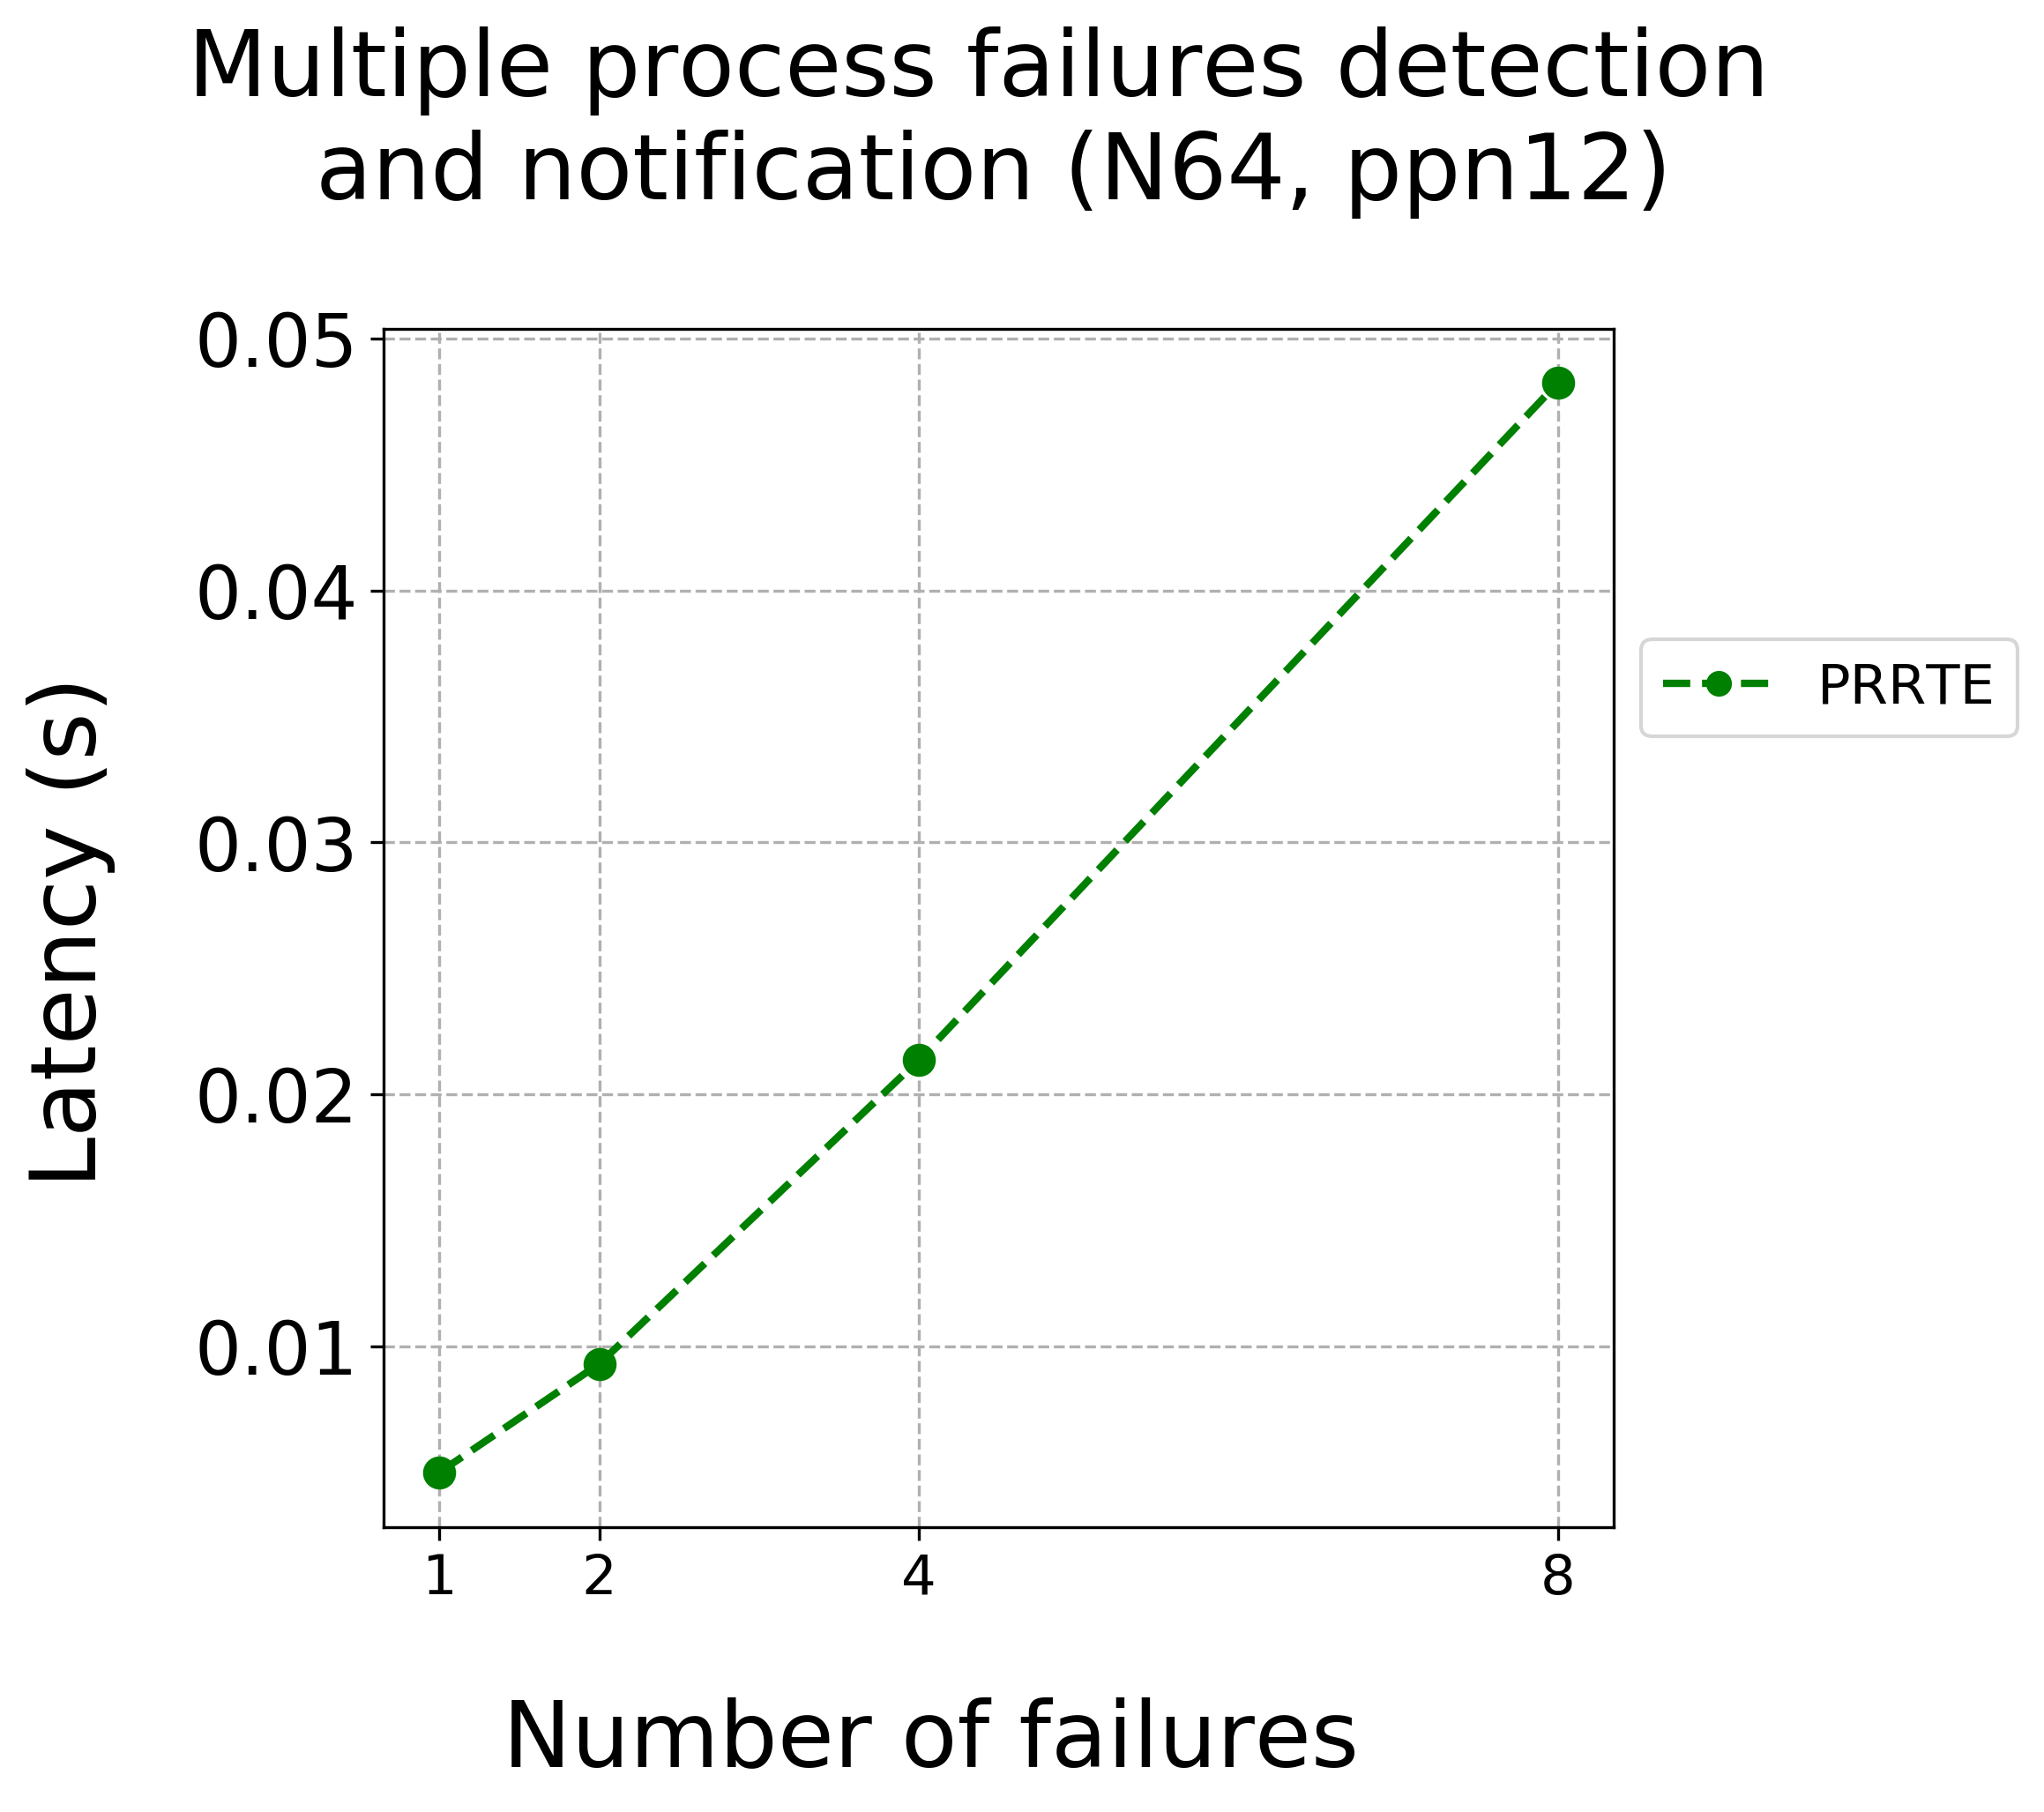
\includegraphics[width=\linewidth]{multi_failures.png}
  \caption{Multiple process failures at the same time}
\end{figure}

\begin{figure}[h]
  \centering
  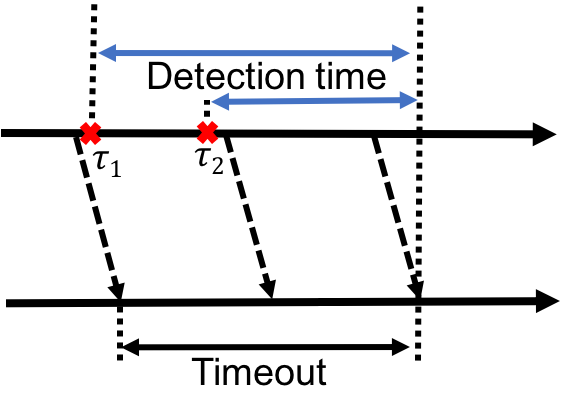
\includegraphics[width=0.8\linewidth,frame]{failure_detection.png}
  \caption{Multiple process failures at the same time}
\end{figure}

\section{Application}


\section{Conclusion}
Failure detection and propagation is a critical service for any fault tolerate systems. The process and node failure detection strategy presented in this work depends on heartbeats and timeouts,  
\section{CCS Concepts and User-Defined Keywords}

\subsection{Inline (In-text) Equations}
\subsection{Display Equations}
A numbered display equation---one set off by vertical space from the
text and centered horizontally---is produced by the \textbf{equation}
environment. An unnumbered display equation is produced by the
\textbf{displaymath} environment.

Again, in either environment, you can use any of the symbols
and structures available in \LaTeX\@; this section will just
give a couple of examples of display equations in context.
First, consider the equation, shown as an inline equation above:
\begin{equation}
  \lim_{n\rightarrow \infty}x=0
\end{equation}
Notice how it is formatted somewhat differently in
the \textbf{displaymath}
environment.  Now, we'll enter an unnumbered equation:
\begin{displaymath}
  \sum_{i=0}^{\infty} x + 1
\end{displaymath}
and follow it with another numbered equation:
\begin{equation}
  \sum_{i=0}^{\infty}x_i=\int_{0}^{\pi+2} f
\end{equation}
just to demonstrate \LaTeX's able handling of numbering.

\section{Citations and Bibliographies}

\section{Acknowledgments}

\section{Appendices}

If your work needs an appendix, add it before the ``\verb|\end{document}|'' command at the conclusion of your source document. 

Start the appendix with the ``\verb|appendix|'' command:
\begin{verbatim}
  \appendix
\end{verbatim}
and note that in the appendix, sections are lettered, not numbered. This document has two appendices, demonstrating the section and subsection identification method.

\section{SIGCHI Extended Abstracts}

The ``\verb|sigchi-a|'' template style (available only in \LaTeX\ and not in Word) produces a landscape-orientation formatted article, with a wide left margin. Three environments are available for use with the ``\verb|sigchi-a|'' template style, and produce formatted output in the margin:
\begin{itemize}
\item {\verb|sidebar|}:  Place formatted text in the margin.
\item {\verb|marginfigure|}: Place a figure in the margin.
\item {\verb|margintable|}: Place a table in the margin.
\end{itemize}

%
% The acknowledgments section is defined using the "acks" environment (and NOT an unnumbered section). This ensures
% the proper identification of the section in the article metadata, and the consistent spelling of the heading.
\begin{acks}
\end{acks}

%
% The next two lines define the bibliography style to be used, and the bibliography file.
\bibliographystyle{ACM-Reference-Format}
\bibliography{sample-base}

% 
% If your work has an appendix, this is the place to put it.
\appendix

\section{Research Methods}

\subsection{Part One}

Lorem ipsum dolor sit amet, consectetur adipiscing elit. Morbi malesuada, quam in pulvinar varius, metus nunc fermentum urna, id sollicitudin purus odio sit amet enim. Aliquam ullamcorper eu ipsum vel mollis. Curabitur quis dictum nisl. Phasellus vel semper risus, et lacinia dolor. Integer ultricies commodo sem nec semper. 

\subsection{Part Two}

Etiam commodo feugiat nisl pulvinar pellentesque. Etiam auctor sodales ligula, non varius nibh pulvinar semper. Suspendisse nec lectus non ipsum convallis congue hendrerit vitae sapien. Donec at laoreet eros. Vivamus non purus placerat, scelerisque diam eu, cursus ante. Etiam aliquam tortor auctor efficitur mattis. 

\section{Online Resources}

Nam id fermentum dui. Suspendisse sagittis tortor a nulla mollis, in pulvinar ex pretium. Sed interdum orci quis metus euismod, et sagittis enim maximus. Vestibulum gravida massa ut felis suscipit congue. Quisque mattis elit a risus ultrices commodo venenatis eget dui. Etiam sagittis eleifend elementum. 

Nam interdum magna at lectus dignissim, ac dignissim lorem rhoncus. Maecenas eu arcu ac neque placerat aliquam. Nunc pulvinar massa et mattis lacinia.

\end{document}
